\pdfoutput=1
\documentclass[11pt,a4paper]{article}
\usepackage[T1]{fontenc}
\usepackage[utf8]{inputenc}
\usepackage{lmodern}
\usepackage[margin=25mm,headheight=14pt]{geometry}
\usepackage{amsmath,amssymb,mathtools}
\usepackage{graphicx,booktabs,tabularx,longtable,array}
\usepackage{enumitem}
\usepackage{listings}
\usepackage{tikz}
\usetikzlibrary{arrows.meta,positioning,calc,fit,backgrounds,shapes.geometric}
\usepackage{microtype}
\usepackage{fancyhdr}
\usepackage{placeins}
\usepackage{xurl}
\usepackage[numbers,sort&compress]{natbib}
\usepackage[hidelinks,pdfusetitle]{hyperref}
\usepackage{bookmark}
\usepackage{tocloft}
\setlength{\cftbeforesecskip}{3pt}
\setlength{\parskip}{0.35em}
\setlength{\parindent}{1.15em}
\setlength{\emergencystretch}{2em}
\setlist{itemsep=0.25em,topsep=0.5em}
\renewcommand{\arraystretch}{1.16}
\pagestyle{fancy}
\fancyhf{}
\fancyhead[L]{\small Superscalar NPU Architecture}
\fancyhead[R]{\small Technical Article}
\fancyfoot[C]{\thepage}
\lstset{basicstyle=\small\ttfamily,breaklines=true,columns=fullflexible,keepspaces=true,showstringspaces=false,frame=none}
\newcommand{\ssnpu}{Superscalar NPU}
\newcommand{\code}[1]{\texttt{#1}}
\title{Superscalar NPU Architecture\\\large Eight Problems in Coordination, Representation, and Progress}
\author{Technical article for the EFCL Zurich workshop}
\date{Research and architecture snapshot: 7 October 2026\\Review draft}
\begin{document}
\maketitle
\begin{abstract}
A matrix accelerator is useful only when its surrounding system can deliver ready operands, perform non-matrix work, retain the right values, and complete the resulting effects. This article develops eight architectural problems that arise in that surrounding system: matrix--vector coordination; latency hiding and storage lifetime; mixed precision, layout, and scale handling; irregular access and atomic updates; reductions along a tensor's tail axis; scalar and event orchestration; precise state and memory ordering; and forward progress under finite resources. For each problem, we examine the responsibilities assigned to algorithms, instruction sets, compilers, runtime software, and hardware in NVIDIA GPUs, Ascend, TPU, Tenstorrent dataflow machines, and a proposed Superscalar NPU. CPU SIMD and published Groq designs provide additional comparisons where their mechanisms illuminate a particular question. The central claim is conditional: bounded dynamic dependency and resource management can reduce coordination work or exposed waiting when useful independent work exists, but its benefit must cover the added state, arbitration, movement, recovery, and progress machinery. Exact numerical and ownership contracts constrain the admissible schedules. Public specifications, version-scoped implementation observations, and proposed mechanisms are kept distinct. This article supplies no new benchmark, silicon measurement, or physical power, performance, and area result.
\end{abstract}
\setcounter{tocdepth}{1}
\tableofcontents
\clearpage
\section{The architectural question}
\label{sec:introduction}

The useful work of a neural processor is seldom one isolated matrix product. A matrix result may feed normalization, indexing, selection, format conversion, another matrix product, or communication with another device. These stages differ in execution width, latency, physical layout, numerical behavior, and ownership. Their interfaces can therefore determine an operator's latency even when the individual arithmetic engines are fast. An architecture must decide when a value is ready, where it lives, who may overwrite it, and which agent can advance the next dependency. These decisions remain necessary whether they are expressed in a compiler schedule, a GPU kernel, a dataflow protocol, or a dynamic scheduler.

This article asks whether a bounded superscalar organization is a useful way to manage some of those decisions in an NPU. Here, ``superscalar'' denotes the possibility of identifying independent ready operations within a finite window and issuing them to available resources. The term does not imply an unbounded instruction window, a CPU-sized general-purpose core, unrestricted speculative memory execution, or a thread context for every tensor element. The proposed programming surface combines scalar control with shaped, typed Tiles. Hardware can track operation dependencies and the availability of finite execution and storage resources. A Tile is an architectural value with a descriptor and a logical valid region; it is not necessarily one indivisible physical transfer, execution step, or storage allocation.

The proposal must be judged against competent alternatives. GPU kernels can distribute control among threads and specialized warps, use asynchronous matrix and copy engines, and compile sophisticated software pipelines. Ascend exposes matrix/vector pipelines, local memories, queues, and events whose composition depends on the product. TPU combines compiler-directed placement with scalar, vector, matrix, and DMA facilities, including low-level programmable asynchronous pipelines. Tenstorrent makes data-movement and compute roles, buffers, and explicit communication central to the programming model. Static scheduling can eliminate substantial dynamic control when shapes, routes, and execution times are predictable. Dynamic scheduling can exploit readiness variation only when work is present and admissible. Neither fact establishes a universal winner.

\subsection{A running example with explicit boundaries}

For the dense example, let a tile of queries $Q\in\mathbb{R}^{M\times D}$ attend to keys $K\in\mathbb{R}^{N\times D}$ and values $V\in\mathbb{R}^{N\times D_v}$. The logical computation is
\begin{align}
 S &= \alpha QK^T + B, \\
 P_{ij} &= \frac{\exp(S_{ij}-m_i)}{\sum_{k=0}^{N-1}\exp(S_{ik}-m_i)},\qquad
 m_i=\max_{0\leq k<N}S_{ik},\\
 O &= PV.
\end{align}
Here $B$ represents an explicitly defined bias or masking rule. The equations describe real-arithmetic intent. A complete implementation additionally chooses input, accumulator, and output types, rounding and exceptional-value behavior, a permitted reduction order, and handling of empty or fully masked rows. These choices affect both numerical results and the schedules that are legal.

The matrix stages produce and consume blocks of scores or probabilities. The middle stage performs reductions and elementwise functions, and it may require retaining scores, exponentials, or partial statistics. If $M$ is small, the implementation has fewer independent rows with which to cover these dependencies. This is a stated low-concurrency case, not a claim that every decoding workload has low concurrency: batch size, heads, parallel sequences, splitting, and device partitioning can all supply more work. Even with many rows, limited storage can prevent all of that work from being resident simultaneously.

Attention does not stand in for every workload. Indexed accumulation is used separately to study irregular access and collisions in Section~\ref{sec:u004}. A producer--communication--consumer pipeline is used to study events and bounded resources in Sections~\ref{sec:u006}--\ref{sec:u008}. Their control and numerical requirements differ, so an optimization valid for a dense attention tile cannot automatically be transferred to a sparse update or a distributed protocol.

\subsection{Eight questions rather than eight mechanisms}

The questions organize the argument because each exposes a distinct obligation:
\begin{enumerate}[label=\textbf{U00\arabic*},leftmargin=4.8em]
 \item Which coordination granularity preserves useful overlap between matrix, vector, and movement stages?
 \item During which part of a value's lifetime must scarce payload storage actually be occupied?
 \item Which format, layout, packing, and scale work remains after competent optimization?
 \item Who handles data-dependent addresses, sparse structure, collisions, and the transition back to regular compute?
 \item Where does a reduction exchange values and retain state, and what numerical order may it use?
 \item Which agent advances scalar submission and completion events while compute is busy?
 \item What state, attribution, visibility, and ordering contracts make asynchronous failures understandable?
 \item Why can admitted work eventually finish when every queue, buffer, and context is finite?
\end{enumerate}
Renaming, partial readiness, late binding, extra scalar contexts, or event offload are possible answers to parts of these questions. They are not premises from which a favorable comparison may be derived. In particular, a scheduling optimization that shortens one wait can lengthen a value's storage lifetime, increase conversion traffic, or obstruct the agent needed to release capacity. The final evaluation must close those loops across the whole core.

\subsection{The conditional thesis}

The working hypothesis is that the gap between \emph{semantic dependencies} and \emph{conservative software coordination} can sometimes be usefully managed by bounded hardware state. If a consumer needs only a defined subset of a producer's output, a correct partial-readiness contract may release it sooner. If a long-latency request need not immediately occupy its final compute storage, separate request identity and physical binding may reduce occupancy. If an independent operation is ready while another waits, resource-aware issue may preserve utilization without an explicit software role split.

Each proposition has a corresponding obligation. Partial readiness requires exact subvalue validity and alias rules. Delayed binding requires a feasible destination or return path. Dynamic issue requires dependency checks, finite queues, and fair selection. Completion requires safe publication and release. Precise recovery may need retained versions or delayed externally visible effects. The design is attractive only where these obligations can be met for less total cost than the coordination or waiting they replace. This is an architectural argument and an evaluation agenda, not a measured claim of improvement.

\section{Evidence and comparison method}
\label{sec:method}

\subsection{Four kinds of statements}

The article distinguishes four evidence levels. A \emph{public contract} specifies software-visible legality, numerical behavior, ordering, or supported use. A \emph{pinned implementation observation} establishes that a particular source revision contains a mechanism or lowering path, within its reviewed scope. A \emph{reported measurement} belongs to the authors, configuration, and methodology of the cited study; it is not a measurement performed for this article. A \emph{conditional design inference} explains what a mechanism could do if its stated assumptions hold. A future design alternative belongs to the last category until an implementation and validation establish more.

These levels are not interchangeable. An opcode in a specification does not prove a production compiler can emit it, that a model computes it accurately, that RTL implements it, or that silicon achieves a particular rate. A compiler recognizer's limited coverage does not shrink an ISA's architectural expressibility. A functional simulation establishes neither a cycle count nor a clock frequency. A timing model's host execution speed is not the modeled machine's performance. An area estimate for one selector is not a whole-core PPA result.

The Superscalar NPU discussion uses the public PTO contract where available and the bounded project-inspection records assembled with the workshop source packet. The timing-model and typed bring-up records concern separate implementation paths; they must not be combined into one demonstrated complete-core implementation. Their inspection supports functional statements about dependency, ownership, and recovery structures, rather than a physical block diagram with verified area or timing. Public documentation whose branch or \texttt{latest} path can change is access-dated; exact revisions are used for claims that depend on a particular contract.

The target architecture includes functionality in submitted integration work once that work is merged. A pending change is therefore not described as architecturally nonexistent merely because of its merge status. At the same time, target intent does not establish new-head validation. Date-stamped implementation notes are retained where they explain a real limitation; they do not define the thesis. No private implementation sources or source-location maps are reproduced.

\subsection{Comparison across five layers}

A comparison begins with the same logical workload and numerical contract, then records where each responsibility is placed.
\begin{description}[style=nextline,leftmargin=0em,labelwidth=0em]
 \item[Algorithm.] Define decomposition, independent work, sparse representation, reduction order, and required results. Algorithmic changes that reduce useful work or alter accuracy must be exposed rather than credited to scheduling alone.
 \item[Instruction set or programming contract.] Specify which operands, layouts, masks, types, atomics, synchronization scopes, and asynchronous lifetimes the interface permits. A high-level API can expand to many instructions; an ISA instruction can execute for many cycles.
 \item[Compiler and kernel.] Record tiling, vectorization, role assignment, layout propagation, prefetch distance, conversion placement, and inserted synchronization. Compare optimized kernels, including transformations that eliminate or amortize apparent source-level overhead.
 \item[Runtime and libraries.] Include allocation, launch, communicator construction, buffer pools, event namespaces, library composition, device placement, and teardown. Setup can be amortized across repeated calls, but still matters for short or infrequent work.
 \item[Hardware.] Identify the execution, storage, dependency, arbitration, movement, and completion functions that must exist. An undocumented internal circuit remains unknown; it is not assumed absent.
\end{description}

For example, a direct Tile reduction and a warp shuffle sequence can express the same mathematical operation at different abstraction levels. Counting one mnemonic against several source operations measures interface compression, not necessarily execution cost. Conversely, placing an entire row in one thread can remove communication that a nominally wider primitive would otherwise need. Ownership and lowering matter as much as the operation name.

\subsection{A whole-core cost ledger}

Let a workload execution perform useful work $W$ and take end-to-end time $T$. Useful throughput is $W/T$, with $W$ defined consistently across the alternatives. Reported utilization must name its denominator: a matrix unit's peak, an instruction issue rate, a memory bandwidth, or another resource. A high matrix utilization can coexist with poor task latency or excess energy if additional work was introduced to keep the matrix unit busy.

A useful accounting record contains at least the following quantities:
\begin{equation}
 \mathcal{C}=\bigl(T,\ W/T,\ S(t),\ D,\ C_{\rm ctrl},\ A,\ P,\ E,\ f,\ \mathcal{S},\ \mathcal{L}\bigr).
\end{equation}
Here $S(t)$ is storage occupancy over time, $D$ is movement at each relevant interface, $C_{\rm ctrl}$ is control state and work, $A$ is area, $P$ is power, $E$ is energy, $f$ is attainable clock frequency, and $\mathcal{S}$ and $\mathcal{L}$ denote required safety and liveness properties. This tuple is a ledger, not a scalar objective with invented weights. The article can reason about functional obligations and derived byte counts without having measured every component. Unmeasured components must remain unmeasured.

For a conservative first-order performance bound, let $W_r$ be the work offered to resource $r$ and $\mu_r$ an upper bound on its service capacity in the stated analytical model and access pattern. A measured average rate alone need not bound short bursts. Ignoring setup and interference gives
\begin{equation}
 T\ \geq\ \max_r\frac{W_r}{\mu_r},\qquad
 T\ \geq\ T_{\rm dependency}.
 \label{eq:resource-bound}
\end{equation}
These lower bounds do not imply that all resources can operate at their isolated peaks simultaneously. Shared ports, banking, issue bandwidth, and live storage can couple them. Overlap shortens exposed elapsed time only if those coupled constraints allow concurrent execution. It does not make the overlapped arithmetic, traffic, or energy disappear.

\subsection{Control functions to account for}

A dynamic core may require a front end, finite issue queues, dependency tags, rename mappings, generation counters, readiness bits, issue selection, storage admission, bank arbitration, and completion/retirement state. The inspected timing-model record includes examples of such functions but does not verify a particular Age Matrix selector or exact physical organization. A CPU-style speculative memory subsystem is not assumed. The typed bring-up path has its own identity, binding, completion, and recovery contracts, which require separate validation.

The alternatives also contain control. GPUs maintain execution state, scoreboards, eligible-warp selection, barriers, and asynchronous pipeline ownership. Ascend APIs expose queues and events around hardware engines. TPU compilers plan lifetimes and DMA synchronization while hardware still advances transfers and execution. Tenstorrent controllers and circular-buffer protocols manage readiness and ownership. Published deterministic streaming designs still need instruction execution, routing, timing alignment, and synchronization. It would be misleading to compare named blocks on one side with an empty box labeled ``static'' on the other.

The important question is which control can be eliminated by static knowledge, which is amortized over larger work, which is hidden behind independent activity, and which remains on the critical path. These categories are used throughout the chapters. They allow a favorable case to be stated without claiming that its mechanism has no cost.

\section{U001 Hybrid matrix and vector coordination}
\label{sec:u001}

A matrix engine can finish useful work only as quickly as the surrounding computation supplies its inputs and consumes its outputs. Attention makes this dependence particularly visible: a matrix multiplication produces scores, vector and reduction operations turn the scores into probabilities, and another matrix multiplication consumes them. An accelerator therefore needs more than a fast matrix datapath. It needs an execution contract that connects different operation shapes, readiness conditions, storage owners, and completion events without imposing avoidable waiting. The question in U001 is which granularity exposes useful overlap, who manages that overlap, and what the resulting control costs are.

This is a mechanism comparison. The NVIDIA case is principally Hopper and a pinned FlashAttention-3 kernel; a separate paragraph identifies a relevant Blackwell change. Ascend A2 and the newer 3510 architecture are kept distinct. The TPU case uses the public Pallas programming model rather than an invented description of a proprietary instruction scheduler. Tenstorrent is considered through its documented compute and circular-buffer interfaces. Our superscalar NPU, abbreviated SSNPU, is discussed through the supplied source-inspection record of a particular timing model, not as measured silicon. Published Groq designs provide a further comparison point. None of the mechanisms described here establishes a performance ordering between platforms.

\subsection{The algorithm creates several different dependencies}

For one query block, let $Q\in\mathbb{R}^{B_q\times d}$ and let the $j$th key and value blocks be $K_j\in\mathbb{R}^{B_k\times d}$ and $V_j\in\mathbb{R}^{B_k\times d_v}$. The score block is
\begin{equation}
 S_j=\alpha QK_j^{\mathsf T}+M_j,
\end{equation}
where $M_j$ expresses the selected mask. A convenient online formulation retains a row maximum $m_j$, a row denominator $\ell_j$, and an unnormalized output accumulator $O_j$. With rowwise broadcasting understood, one iteration is
\begin{align}
 m_j &= \max\bigl(m_{j-1},\operatorname{rowmax}(S_j)\bigr),\\
 a_j &= \exp(m_{j-1}-m_j),\qquad
 P_j=\exp(S_j-m_j),\\
 \ell_j &= a_j\ell_{j-1}+\operatorname{rowsum}(P_j),\\
 O_j &= a_jO_{j-1}+P_jV_j.
 \label{eq:u001-online-attention}
\end{align}
For rows with valid scores, the recurrence starts from $m_0=-\infty$, $\ell_0=0$, and $O_0=0$, with the first valid block handled consistently with those initial values. The final output divides each row of $O_j$ by its corresponding denominator. This mathematical formulation does not prescribe a particular instruction schedule or numerical implementation. Input precision, accumulator precision, approximation of exponential, exceptional values, and the treatment of fully masked rows must be specified separately.

There are at least three kinds of dependence in this small program. Within a block, probabilities require the appropriate maximum, and the contribution to the output requires those probabilities. Across blocks, the running state connects successive iterations. Across query rows or independent heads, substantial work can be independent. These distinctions explain why both of the following statements can be true: a score block cannot skip its softmax dependencies, and a kernel can execute some matrix work concurrently with softmax work. FlashAttention-3 explicitly exploits asynchronous matrix execution and rearranged block scheduling to obtain such overlap on Hopper. Its reported performance is evidence for its evaluated configurations, not a transferable result for the SSNPU or for every attention shape.~\citep{u001-fa3}

The decomposition also prevents a misleading account of ``the vector stage.'' Row maximum, exponential, sum, broadcast, output rescaling, and normalization have different input requirements. A row maximum can accumulate partial maxima as score fragments arrive, but its final value requires every active fragment in that reduction domain. An elementwise operation with independent inputs may become eligible much earlier. The relevant dependency is therefore a relation between producer regions and consumer operations, not merely an arrow between two large boxes labelled matrix and vector.

\subsection{Five granularities must be distinguished}

We use five separate meanings of granularity. \emph{Semantic work granularity} is the operation the program expresses, such as a score tile or row reduction. \emph{Dispatch granularity} is the unit admitted or selected by a scheduler. \emph{Readiness granularity} is the smallest region for which the implementation can establish that required data are valid. \emph{Synchronization granularity} is the participating group and event scope used to communicate this fact. \emph{Transfer granularity} describes a memory request or movement unit. These quantities can differ within one operation and can change between generations of the same product.

For example, the supplied benchmark inspection identifies a group score tile with $B_q=B_k=128$, but the selected four-PE kernel gives each PE a $32\times128$ FP32 score shard. The group FP32 payload is $64$ KiB, the per-PE payload is $16$ KiB, and a modeled vector readiness cell is $128$ bytes. A cell contains $32$ FP32 values by capacity; it is neither the whole vector operation nor evidence that those values execute in one cycle. Doubling $B_k$ doubles the shard's logical byte count without proving that dispatch or readiness granularity changes. These are source-derived geometry observations and arithmetic, not dynamic instruction counts.~\citep{u002-benchmark-fa,u001-ssnpu-audit}

A corresponding NVIDIA example must name its own layer. A full warp executing one FP32 operation per active thread spans $128$ bytes per operand when all $32$ threads participate. Hopper WGMMA instead uses a warpgroup of $128$ cooperating threads. For a dense BF16 $m64n128k16$ operation, the logical inputs contain $2$ KiB of A and $4$ KiB of B, while an FP32 accumulator contains $32$ KiB. These figures describe matrix shapes and representations, not memory transactions or a universal software tile.~\citep{u001-ptx} Equal byte counts between an SSNPU cell and a warp operand establish no equivalence between their scheduling semantics.

The historical Ascend attention design also identifies an operator whose vector piece is $8\times1024$ FP32, or $32$ KiB. Its significance is a buffer and decomposition choice in that operator, not a fixed hardware asynchronous scheduling quantum.~\citep{u001-ascend-fa-design} Comparing this piece directly with a GPU warp or a $128$-byte readiness cell mixes semantic work, capacity, and execution participation. A meaningful comparison first identifies the producer region, the required consumer region, and the actual operation that moves or consumes it.

\subsection{What finer readiness can and cannot change}

Consider an illustrative producer that makes four independently usable regions available at times $t_1<t_2<t_3<t_4$. A consumer requires only the first region. If the interface exposes one whole-tile completion event, the earliest dependency-permitted start is $t_4$. If it exposes correct region readiness, that bound becomes $t_1$. The opportunity is $t_4-t_1$, but the actual improvement can be smaller or zero: the execution unit may be occupied, a destination may be unavailable, or bank conflicts may prevent admission. This is a dependency argument, not a prediction of observed cycles.

For a consumer $v$, write its earliest admissible start schematically as
\begin{equation}
 s_v\geq\max\{r_v,\ d_v,\ e_v,\ b_v,\ o_v\},
 \label{eq:u001-admission}
\end{equation}
where $r_v$ is the latest required input-ready time, $d_v$ is destination availability, $e_v$ is execution-resource availability, $b_v$ is the relevant bank or port availability, and $o_v$ expresses ordering constraints. Replacing whole-tile readiness with region readiness changes $r_v$ only. A scheduling proposal that ignores the other terms can substantially overstate its benefit.

\begin{figure}[tb]
\centering
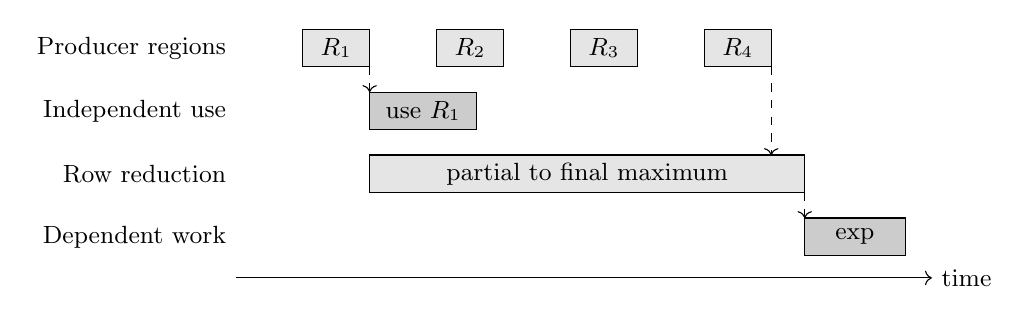
\begin{tikzpicture}[x=0.85cm,y=0.8cm, every node/.style={font=\small}]
 \node[anchor=east] at (0,3) {Producer regions};
 \node[anchor=east] at (0,2) {Independent use};
 \node[anchor=east] at (0,1) {Row reduction};
 \node[anchor=east] at (0,0) {Dependent work};
 \draw[->] (0,-0.65)--(10.4,-0.65) node[right] {time};
 \foreach \x/\n in {1/1,3/2,5/3,7/4} {
   \draw[fill=black!10] (\x,2.7) rectangle (\x+1,3.3);
   \node at (\x+0.5,3) {$R_{\n}$};
 }
 \draw[fill=black!20] (2,1.7) rectangle (3.6,2.3);
 \node at (2.8,2) {use $R_1$};
 \draw[->,dashed] (2,2.7)--(2,2.3);
 \draw[fill=black!10] (2,0.7) rectangle (8.5,1.3);
 \node at (5.25,1) {partial to final maximum};
 \draw[->,dashed] (8,2.7)--(8,1.3);
 \draw[fill=black!20] (8.5,-0.3) rectangle (10,0.3);
 \node at (9.25,0) {exp};
 \draw[->,dashed] (8.5,0.7)--(8.5,0.3);
\end{tikzpicture}

\caption{Conceptual readiness relationships. Region arrival can advance independent work and partial reduction, while the final maximum still gates dependent exponentials in this formulation. Horizontal distances are illustrative and do not represent measured timing or a particular architecture.}
\label{fig:u001-readiness}
\end{figure}

Now make each region one quarter of a softmax row. Partial maxima can begin early, but exponentiating every quarter relative to the final block maximum cannot begin merely because the first quarter exists. One may use an alternative online update scheme, but then its additional rescaling and retained state belong in the accounting. Alternatively, make each region a complete subset of rows. Those rows can complete their reductions without waiting for unrelated rows, provided the producer really finishes the corresponding reduction dimension and the consumer mapping supports that partition. Fine readiness is valuable when it matches the algorithm's independence; an arbitrary byte partition does not create such independence.

This distinction also matters for low-concurrency workloads. Let $N$ be the number of useful pipeline iterations, $T_{\mathrm{fill}}$ the initial preparation interval, $I$ the achievable steady-state initiation interval, and $T_{\mathrm{drain}}$ the remaining work after the final iteration is admitted. An idealized latency decomposition is
\begin{equation}
 T(N)=T_{\mathrm{fill}}+(N-1)I+T_{\mathrm{drain}},\qquad N\geq1.
\end{equation}
Reducing $I$ has little leverage when $N=1$. Reducing a real dependency on the first or last tile can instead affect fill or drain. Conversely, splitting work more finely can increase setup, events, and intermediate storage. A claim about short-task latency must state batch size, heads, sequence lengths, dimensions, masking, and partitioning; it cannot be inferred from a steady-state utilization number or generalized to all decode.

\subsection{NVIDIA assigns roles in software and eligibility in hardware}

Hopper exposes asynchronous matrix and transfer facilities that a compiler or kernel author can compose into a fused pipeline. TMA moves appropriately described tensor data, while warps and warpgroups perform different producer and consumer roles. Hardware schedules eligible resident work and enforces exposed completion mechanisms; software determines tile shapes, layouts, stage count, role assignment, and synchronization placement. The Hopper tuning guide describes the hardware facilities, while a concrete kernel establishes how they are used.~\citep{u001-hopper}

CUTLASS's Hopper organization makes this division explicit. Producer warps wait for an empty shared-memory stage, initiate a transfer, and associate arrival with the stage's completion state. Consumer warps wait for the stage to become full, issue matrix work, and release the stage when it can safely be overwritten.~\citep{u002-cutlass} This is already dynamic readiness-based coordination at the software-defined stage boundary. It should not be described as a machine that relies entirely on a fixed cycle schedule, nor should ready-warp scheduling be equated with unrestricted CPU-style speculative out-of-order execution.

The useful opportunity is to overlap independent stages and to use different engines concurrently. The cost includes producer instructions, barrier state, register and shared-memory capacity, layout preparation, and constraints on resident work. More software stages can improve latency tolerance while reducing other forms of concurrency. An application-level runtime can also select different decompositions: TensorRT-LLM documents multi-block attention choices intended to provide additional work when batch-times-head count is small. That option introduces its own partial-result and coordination costs; it is a relevant baseline for a low-concurrency comparison, not a guarantee of lower latency.~\citep{u001-trt-attention}

The generation boundary is important. Blackwell SM100 introduces the \texttt{tcgen05} family with single-thread matrix instruction launch and Tensor Memory for accumulators.~\citep{u001-tcgen05} FlashAttention-4 describes algorithm and pipeline changes for that organization.~\citep{u001-fa4} Therefore the number of threads participating in Hopper WGMMA cannot be presented as an immutable property of NVIDIA matrix execution. A fair comparison may choose Hopper for its pinned implementation evidence, but it must say so rather than treating an older interface as the only available GPU approach.

\subsection{Ascend exposes pipeline and inter-core coordination}

In the A2 separated organization, Cube and Vector cores have independent scalar control. The documented architecture distinguishes Cube operand and accumulator storage from the Unified Buffer used by Vector work; movement engines connect the relevant storage levels. Its instruction queues and synchronization interfaces permit overlap across pipelines while preserving dependencies. GM-addressed exchange is not synonymous with a mandatory HBM round trip because the architecture documents L2 caching of DMA traffic.~\citep{u001-ascend-basic}

At the algorithm and compiler level, host tiling and kernel code choose which Cube region becomes which Vector pieces, which layouts are used, and how much state remains resident. At the API level, queues and events identify ownership and inter-pipeline dependencies. Hardware executes those operations and supplies the movement and event mechanisms. A larger Cube tile can amortize setup and reuse operands, while smaller Vector pieces can begin useful work incrementally. Neither choice is free: exchanged data, local capacity, events, and the number of simultaneously live intermediates constrain the resulting schedule.

The \texttt{TQue} contract is especially relevant because it separates a queue of tensor references from the number of physical buffers allocated for that queue. Queue depth and multibuffering count answer different questions; increasing one does not automatically increase the other.~\citep{u002-ascend-tque} This is a concrete example of why an API-level queue size cannot serve as a universal hardware issue granularity. Similarly, an operator's $32$ KiB vector allocation is not evidence that every useful handoff waits for $32$ KiB.

For architecture 3510, the official specification identifies additional L0C-to-UB and UB-to-L1/L1-to-UB paths, as well as SSBuffer for AIC--AIV communication. It also documents SIMD register-based execution and SIMT hardware, including warp schedulers, so an A2 description must not be treated as the execution model of every Ascend generation.~\citep{u001-ascend-3510} These changes alter the possible handoff and control costs. The present comparison does not project A2's paths onto 3510, infer throughput from the existence of a path, or assume that every software release uses it optimally. The open measurement question is which decomposition sustains useful overlap for the selected shapes after exchange and control costs are included.

\subsection{TPU gives the compiler a larger scheduling responsibility}

Pallas describes a TPU TensorCore with scalar, vector, and matrix execution resources that can operate asynchronously under compiler management. The programmer sees a predominantly single-threaded program and can express DMA, memory spaces, and pipeline structure.~\citep{u001-pallas-pipeline} This organization separates an instruction stream's presentation from the concurrency of the engines it controls. A sequential kernel body does not imply that every transfer, matrix operation, and vector operation is serialized to completion.

The compiler and kernel author choose blocking, layout, fusion, and the order of work; explicit buffer and semaphore operations establish important readiness conditions. The documented constraints on blocks and memory spaces, and the distinction between vector and matrix operations, matter when mapping a score tile to reductions.~\citep{u001-pallas-details} A pipeline that overlaps HBM-to-VMEM DMA with computation does not by itself establish that the score matrix multiply overlaps every softmax stage. That requires an effective schedule and sufficiently independent work on the relevant engines.

A static description of that schedule should not be caricatured as an inability to handle runtime variation. Pallas supports scalar-prefetched information for runtime block indexing in documented sparse patterns.~\citep{u001-pallas-sparse} Runtime completion and buffering can handle lateness by waiting rather than by corrupting data. The likely tradeoff, as a design inference, is between predictable scheduling with relatively explicit lifetimes and the ability to exploit unanticipated ready work. Which side matters more depends on shape regularity, memory behavior, the compilation, and available local capacity. It is not determined by the label ``compiler directed.''

\subsection{Tenstorrent separates placement from readiness}

Tenstorrent's Metalium programming model divides work among data-movement and compute roles. RISC-V control processors issue commands; the tensor arithmetic is performed by the corresponding compute engines. Circular-buffer operations coordinate publication, consumption, and available space.~\citep{u001-metalium} Software placement of kernels and streams therefore coexists with runtime readiness and backpressure. A static placement is not necessarily a cycle-by-cycle static execution schedule.

Within Tensix, the matrix engine and vector engine meet through Dst storage. Unpack, math, and pack activities have explicit ownership synchronization; the documented \texttt{tile\_regs\_*} lifecycle separates acquiring compute access, committing results, waiting for packing access, and releasing the resource.~\citep{u001-tensix} The implication for attention is that local ownership can be as important as nominal engine independence. Two operations assigned to different arithmetic facilities may still serialize because their command role, Dst region, or packing path is shared.

The official repository's investigation of SDPA implementation paths distinguishes a non-streaming FP32-Dst path, where the math-thread exponential serializes with matrix work, from a streaming path that issues exponential work from the pack thread.~\citep{u001-tt-sdpa-investigation} This is useful implementation-specific evidence, not proof that all Tensix kernels either overlap or fail to overlap matrix and vector work. The algorithm must still provide independent blocks; the kernel must provide compatible Dst ownership and command sequencing; and L1 circular buffers must support the required run-ahead. Host asynchronous dispatch or replay cannot establish any of those internal overlap properties by itself.

The published Groq TSP designs show a further possible division of responsibility: compiler placement and timing arrange streams between functionally specialized slices, with network synchronization maintaining the timing contract.~\citep{u001-groq2020,u001-groq2022} This can make predictable streaming attractive, but it does not remove the attention dependencies derived above. These published designs are a comparison of contracts, not a description of every current Groq product or a low-concurrency performance verdict.

\subsection{The SSNPU opportunity is bounded dynamic coordination}

The supplied SSNPU audit covers the handwritten TimingSim snapshot at commit \texttt{d5419b3e721d}. It observes logical operand tags, whole-tile readiness, conditional cell readiness, bounded issue queues, resource checks, and physical binding. CUBE selection is gated by dependence, chain order, speculation, and execution or storage resources. VEC selection is organized by execution class and is subject to initiation intervals, destination capacity, and backpressure. Cell-mode vector block entry retains an ordering restriction.~\citep{u001-ssnpu-audit} These facts support a bounded dynamic coordination design; they do not describe unrestricted global out-of-order execution.

The intended division is that software expresses operation geometry, layouts, logical dependencies, and reuse, while the hardware model enforces eligible readiness and resource admission. Conditional cell readiness can lower $r_v$ in Equation~\ref{eq:u001-admission} for supported producer--consumer combinations. It cannot lower the other admission bounds automatically, and an operation requiring whole-tile readiness remains constrained by that contract. The audit does not establish arbitrary nonlinear layouts, arbitrary independent source shapes, or an automatically optimal compiler decomposition.

The corresponding normative design requirement is precise: every early consumer must read the correct generation of every required region, no consumer may observe an unfinished or overwritten value, and issue must respect both program ordering and physical resource ownership. This requirement is independent of the particular mechanism used to implement it. Logical tags, scoreboards, readiness masks, bank reservations, and queue selection are implementation choices that carry state, wiring, arbitration, and verification obligations. An abbreviated source program cannot demonstrate that their total cost is lower than that of explicit software stages.

The target architecture should also be kept distinct from a narrow executable snapshot. Functionality delivered by a submitted change belongs in the after-merge target when the change is integrated; its absence from an earlier experiment does not establish architectural inexpressibility. Conversely, a proposed interface does not prove that the measured path used it. For U001, this distinction requires the exact build and configuration before attributing any overlap to cell readiness, ready bypass, or a particular binding path. TimingSim observations are not evidence of complete RTL integration, clock closure, physical area, or energy.

\subsection{A useful evaluation isolates the source of overlap}

A matched study should retain the same attention semantics and vary query rows, key length, head dimensions, masking, and available independent heads. It should record semantic tiles, per-owner shards, readiness regions, synchronization participants, and transfer units separately. End-to-end latency should include preparation, fill, steady state, and drain. A steady-state engine-utilization trace should identify what useful work overlaps, rather than merely showing two queues nonempty.

For the SSNPU, a readiness-granularity ablation must preserve the rest of the build, resource budget, scheduling options, and numerical path. Otherwise a change attributed to smaller regions may instead come from different reduction ordering, queue policy, or storage capacity. Competent GPU, Ascend, TPU, and Tenstorrent baselines should use their own supported fusion and pipelining facilities. The resulting ledger must include event and issue work, retained payload, extra transfers, mapping and arbitration state, and correctness and progress constraints. Finer granularity is justified when it advances useful admissible work enough to repay those costs; neither finer readiness nor a larger matrix tile is intrinsically better.

\section{U002 Latency hiding and physical storage lifetime}
\label{sec:u002}

Latency hiding requires work to be outstanding before it is needed. It does not follow that every outstanding operation must occupy its eventual compute destination for the whole wait. The distinction is the subject of U002: when must a physical payload location be owned, what state must remain while it is not owned, and when is reuse safe? Compiler lifetime planning, software multibuffering, explicit dataflow queues, and hardware-managed logical-to-physical binding are different answers to this question. Their comparison requires separate accounting for requests, returned data, allocation pools, individual values, and genuinely live compute state.

This distinction is easy to lose in attention. A kernel can prefetch a future K block while retaining Q, running maxima and denominators, an output accumulator, and other K/V blocks being consumed. Some storage contains useful live data; some is reserved for a future arrival; some exists because the enclosing kernel allocated a fixed pool. Reclaiming one consumed K slot does not free the pool, and making part of a score tile readable does not establish that its physical storage can be released one cell at a time. The relevant objective is to reduce avoidable residency while retaining correct ownership and a completion path for every admitted operation.

\subsection{Five intervals describe one asynchronous load}

For a value $i$ with logical payload size $b_i$ and charged physical allocation size $s_i$, distinguish the following intervals. \emph{Request tracking} begins when the system must remember an operation's identity and ends when the associated tracking state is no longer required. \emph{Returned-data residence} covers a response that has arrived but has not yet been placed in or consumed from its next storage location. \emph{Pool allocation} is the interval during which a larger capacity reservation exists. \emph{Value ownership} is the interval during which a particular slot belongs to value $i$ and cannot be overwritten by another value. \emph{Compute-live residence} covers valid payload held in compute-local storage that is still required by remaining consumers. Returned data waiting elsewhere are also logically live; this last category isolates their residency after placement in compute storage. The intervals can overlap. The exact boundaries depend on the interface; these categories are an accounting framework rather than a universal implementation diagram.

Let $a_i$ be physical destination acquisition and $f_i$ safe release. For distinct, non-aliased allocations, let $s_i$ include the physical envelope, padding, and capacity rounding charged to the value. The destination occupancy attributable to values is
\begin{equation}
 D(t)=\sum_i s_i\,\mathbf{1}_{[a_i,f_i)}(t),
 \qquad
 A_D=\int D(t)\,dt=\sum_i s_i(f_i-a_i),
 \label{eq:u002-byte-time}
\end{equation}
where $A_D$ is a byte-time measure. It exposes long avoidable holding intervals, but it is not an area estimate. Physical implementation also depends on peak simultaneous demand, banking, ports, fragmentation, and whether different pools can share capacity. If a fixed pool has capacity $C$, slot reuse can reduce value occupancy within it while leaving the allocated capacity $C$ unchanged.

Similarly, request count $N_{\mathrm{req}}(t)$ is not payload capacity. A request record might hold an address, length, tag, generation, and status rather than a complete data tile. Return buffers can have their own allocation and backpressure rules. If the same physical memory backs several roles, their occupancy must be counted as a union of physical regions rather than summed twice. If they are disjoint, each region's capacity and lifetime belongs in the ledger. Neither ``bytes in flight'' nor ``number of buffers'' is sufficiently precise by itself.

\begin{figure}[tb]
\centering
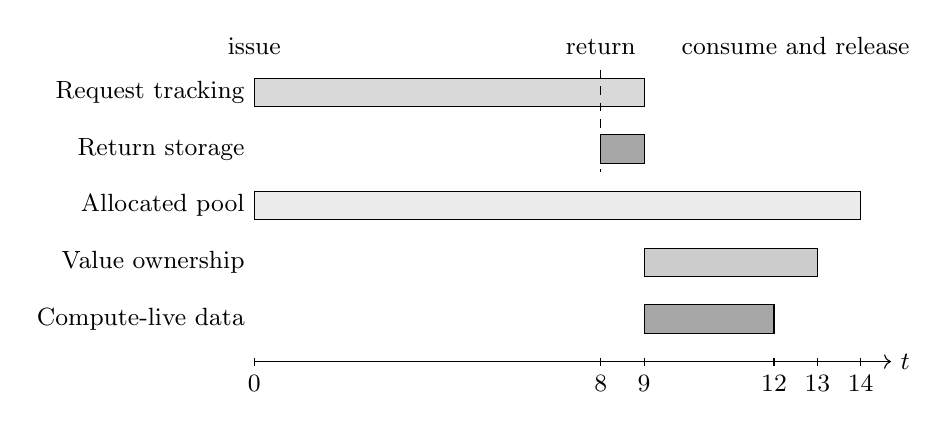
\begin{tikzpicture}[x=0.55cm,y=0.72cm,every node/.style={font=\small}]
 \node[anchor=east] at (0,4) {Request tracking};
 \node[anchor=east] at (0,3) {Return storage};
 \node[anchor=east] at (0,2) {Allocated pool};
 \node[anchor=east] at (0,1) {Value ownership};
 \node[anchor=east] at (0,0) {Compute-live data};
 \draw[fill=black!15] (0,3.75) rectangle (9,4.25);
 \draw[fill=black!35] (8,2.75) rectangle (9,3.25);
 \draw[fill=black!8] (0,1.75) rectangle (14,2.25);
 \draw[fill=black!20] (9,0.75) rectangle (13,1.25);
 \draw[fill=black!35] (9,-0.25) rectangle (12,0.25);
 \draw[->] (0,-0.75)--(14.7,-0.75) node[right] {$t$};
 \foreach \x in {0,8,9,12,13,14} {
  \draw (\x,-0.68)--(\x,-0.82);
  \node[below] at (\x,-0.83) {\x};
 }
 \node[above] at (0,4.5) {issue};
 \node[above] at (8,4.5) {return};
 \draw[dashed] (8,4.4)--(8,2.6);
 \node[above] at (12.5,4.5) {consume and release};
\end{tikzpicture}

\caption{An illustrative late-binding lifecycle. The response arrives at $t=8$, destination ownership begins at $t=9$, the last modeled computation consumes the data by $t=12$, and ownership is released at $t=13$. The enclosing pool remains allocated until $t=14$. These times are invented for explanation; tracking may last longer in other implementations.}
\label{fig:u002-lifetimes}
\end{figure}

For the example in Figure~\ref{fig:u002-lifetimes}, suppose the logical payload and charged allocation are both $16$ KiB. An early-bound destination held from $t=0$ through $t=13$ accounts for $208$ KiB-time units; a destination acquired at $t=9$ accounts for $64$. The difference, $144$ KiB-time units, is an illustrative reduction in that destination's reservation interval. It is not a claim of saved SRAM area or energy. The late-bound design also requires return storage during $[8,9)$, may temporarily hold two copies during movement, and needs mapping and arbitration state. If its enclosing pool is unchanged, physical capacity may be identical. If binding is delayed until $t=11$, the consumer may start later; the smaller destination interval can then accompany worse latency. A residency result must therefore be reported together with completion time and occupancy elsewhere.

\subsection{Outstanding work and live payload impose different bounds}

For a steady stream of fixed-size requests with average request rate $\lambda$ and average request latency $L$, the average outstanding count is $\lambda L$ under the usual stable-flow assumptions. At a delivered byte rate $B$, the associated bandwidth--latency product is $BL$. For variable request sizes, let $\ell$ be per-request latency, with $L=\mathbb{E}[\ell]$. Mean outstanding bytes are $\lambda\mathbb{E}[b\ell]=B L_b$, where $L_b=\mathbb{E}[b\ell]/\mathbb{E}[b]$ is byte-weighted mean latency. This is a statement about outstanding traffic, not proof that $BL$ bytes occupy a particular SRAM. Bytes may still reside at the source, be traversing a network, wait in return storage, or have arrived at their destination. The architecture determines which of these states requires an explicit payload reservation.

An idealized pipeline producing one tile every $I$ time units needs roughly $\lceil L/I\rceil$ requests in flight to cover a fixed latency $L$, before additional constraints are considered. Burstiness and variable service can require more slack or force stalls. A finite queue cannot guarantee a target throughput for arbitrary unbounded delay. Equally, adding destination buffers cannot overcome a sustained bandwidth deficit: if the consumer needs $b/I$ bytes per unit time and the supply can deliver only $B<b/I$, eventual starvation remains.

There is also an independent lower bound from truly live values. For a chosen algorithm and schedule without spilling or recomputation, all values needed by future consumers must remain available somewhere. If $\mathcal{L}(t)$ is the set of such values, then storage across the locations retaining them must accommodate their live payload, with aliases counted once. Late binding can remove an unnecessary pre-arrival destination hold; it cannot remove the information content of $\mathcal{L}(t)$. A different algorithm may reduce this set through streaming, recomputation, or changed accumulation, but its extra compute and traffic must then be charged to that algorithm.

This is why the running state in Equation~\ref{eq:u001-online-attention} matters. A K block can often be released after its last relevant QK use, while an output accumulator and row statistics remain necessary across subsequent KV blocks. Treating all of these as identically short-lived tiles exaggerates what an allocator can reclaim. The meaningful question is which values are held before they are present, after their final use, or in unnecessarily duplicated form, and whether shortening those intervals changes a binding capacity constraint.

\subsection{NVIDIA stage reuse is a complete ownership protocol}

In a Hopper TMA pipeline, shared-memory stages are software-selected destinations. The producer obtains a reusable stage, starts the copy, and allows transfer completion to establish readiness; the consumer waits, uses the data, and releases the stage for another iteration.~\citep{u002-cutlass} Copy completion and consumer completion are different events. Reusing a stage after the first but before the second can overwrite an operand still being read by asynchronous matrix work.

The pinned FlashAttention-3 source illustrates this distinction directly. At revision \texttt{dc8fd708575a}, the K producer acquires its pipeline stage before issuing the TMA copy. In the selected intra-warpgroup-overlap loop, QK for the current block is interleaved with PV for an earlier block. The loop waits for the appropriate matrix progress before releasing K, performs online softmax, then waits for the remaining matrix work before releasing V on the ordinary no-QV path.~\citep{u002-fa3-mainloop} The source establishes distinct K and V lifetimes. It does not establish that every template instantiation uses the same branch or stage geometry.

The compiler and kernel own the stage layout, number of stages, and consumer-release placement; hardware transfer and completion facilities implement the asynchronous operations. TMA's direct movement avoids an intermediate general-purpose-register copy on supported paths.~\citep{u002-cuda-async} That saves a particular movement and register role, but does not establish late physical allocation of the shared-memory destination. Register budgeting is another separate mechanism: PTX's \texttt{setmaxnreg} permits supported redistribution within the CTA register pool.~\citep{u002-setmaxnreg} It would be inaccurate to describe all register ownership as immutable, or to treat register redistribution as shared-memory late binding.

For a matched experiment, the costs include stage capacity, barriers and phase bookkeeping, producer and consumer instructions, resident register requirements, and waiting for reusable stages. More stages can absorb additional latency while reducing the room for other resident work. Private request and response-buffer policies cannot be reconstructed from this API description; they remain unspecified in this comparison. A software-managed stage is a real solution to safe latency hiding, with a different ownership boundary from logical-tag binding.

\subsection{Ascend separates pool creation from tensor reuse}

Ascend C's \texttt{InitBuffer} establishes buffers associated with a \texttt{TPipe}-managed queue or buffer object. The queue form accepts both buffer count and per-buffer length.~\citep{u002-ascend-initbuffer} A tensor allocated from this capacity acquires a slot; queue operations pass its ownership reference between stages. The \texttt{TQue} description explicitly distinguishes queue depth from the number of buffers and describes dequeue as returning a tensor reference rather than copying the data.~\citep{u002-ascend-tque} Thus queue occupancy, pool capacity, and payload movement are separate quantities.

\texttt{FreeTensor} releases a tensor previously obtained through \texttt{AllocTensor}.~\citep{u002-ascend-freetensor} Its name must not be read as proof that the entire physical pool disappears. It permits reuse within that pool; the encompassing management object has a separate lifecycle. At the algorithm level, the kernel decides when a tile's remaining consumers have finished. At the API level, queue and event operations express the necessary handoffs. Hardware movement and execution pipelines perform the underlying work, subject to the chosen generation's storage and transfer paths.

This division supports streaming and multibuffering, but it also places real obligations on the kernel: a queued address must continue to identify the intended data, a stage must not free an input still used by another asynchronous operation, and the next producer must not overwrite a live slot. Buffer count can increase tolerance of variable delays at a capacity cost. Whether a particular operator reduces its pool size or only reuses slots more frequently requires its actual tiling and allocation plan. The public APIs do not establish an issue-time or response-time policy for every hidden hardware buffer.

\subsection{TPU compiler planning can shorten residency}

Pallas exposes VMEM buffers and semaphore-backed asynchronous movement. Its TPU pipeline documentation allows per-argument multibuffering and currently documents two buffers as the default for inputs and outputs.~\citep{u001-pallas-pipeline} That default is a software-interface fact, not a universal TPU hardware capacity. The asynchronous-copy interface separates completion associated with reading the source from completion associated with writing the destination.~\citep{u002-pallas-copy} Neither event, alone, says that all downstream consumers have relinquished ownership.

Compiler management should not be equated with reserving every buffer for a worst-case delay. OpenXLA's memory-space-assignment description, inspected at revision \texttt{82e6c3119a94}, represents a value through allocation sequences and use segments, including prefetch, eviction, and sliced-copy allocations. It explicitly describes sliced copies as a way to defer destination allocation.~\citep{u002-xla-msa} This is a compiler-side mechanism for changing residency intervals. Its presence does not prove that a particular Pallas kernel receives that transformation, or that a target compilation selects the best lifetime plan.

Runtime completion remains relevant even with a planned schedule. The Pallas distributed-computing documentation explains how additional slots permit bounded run-ahead and how receiver-to-sender synchronization prevents overwriting a buffer when devices progress at different rates.~\citep{u002-pallas-distributed} The same distinction between correctness and performance is useful locally: completion and ownership rules prevent a race, while lookahead and buffer depth seek to prevent an idle engine. If a transfer is late, a correct program may wait. A performance plan based on expected latency need not allocate for every conceivable delay in order to remain correct.

The tradeoff is therefore more precise than ``static versus dynamic memory.'' A compiler can shorten a known live range and schedule just-in-time prefetch; a runtime completion mechanism can tolerate variation by delaying progress; hardware-managed binding can choose an acquisition point after observing an event. Each technique may reduce a different form of conservatism. Their costs include planning complexity, explicit synchronization, extra movement, delayed issue, or mapping state. A common workload and generated executable are needed to determine which of these costs dominates.

\subsection{Tenstorrent makes streaming ownership explicit}

Tenstorrent's host circular-buffer interface allocates L1 capacity for the participating cores.~\citep{u002-tt-cb} Within a kernel, reserving space, publishing produced tiles, waiting for available input, and popping consumed tiles describe a value lifecycle inside that capacity. The documented reserve operation waits for sufficient free space without itself advancing the producer pointer.~\citep{u002-tt-reserve} Data arrival does not automatically publish a tile, and a read does not automatically reclaim it. The kernel must perform the matching operations at a safe point.

A representative reader sequence is to reserve an output slot, issue an asynchronous NoC read to that slot, wait for the relevant transfer completion, and publish the tile. The compute side waits for published input and eventually releases the consumed capacity.~\citep{u001-metalium} This exposes both readiness and bounded producer run-ahead. It also exposes the cost of a slow consumer: once the circular buffer is full, the producer waits even if it could otherwise issue more requests. A deeper buffer trades L1 capacity for additional tolerance.

The Wormhole B0 NoC counter specification supplies a particularly useful distinction. A command-control slot can become reusable when the first-hop virtual channel is assigned, while read completion is recorded only after the response data have been written to the return location.~\citep{u002-tt-counters} Command-slot lifetime and payload lifetime therefore differ. This is evidence against treating every outstanding request as a permanently occupied command register, but it is not evidence for a generic late allocator of L1 payload destinations. Likewise, cut-through network movement should not be modeled as a complete tile reservation at every router without a source establishing that organization.

\subsection{SSNPU logical identity can precede physical binding}

The supplied TimingSim inspection observes a distinction between a Tile's virtual identity, including generation, and its physical binding. Ordinary issue-time binding coexists with a conditional real-L2 local-load path that requests destination binding after returned-data readiness; shared staging uses a different path. A failed bind waits for capacity. Bounded request and grant machinery, physical references, consumer checks, aliases, and recovery boundaries participate in safe allocation and release.~\citep{u001-ssnpu-audit} These observations concern the pinned model, not every load or an automatically enabled property of every benchmark.

The architectural opportunity is to keep the dependency identity alive while deferring ownership of a scarce compute-local destination. Software still describes the operation, geometry, reuse, and program dependencies. Hardware-model control can decide when the relevant physical capacity is available, connect the returned value to its logical name, and wake supported consumers. This moves some ownership coordination below the kernel API, but it does not eliminate the ownership protocol. The state now includes mapping and generation information, bind arbitration, reference or alias checks, and the handling of responses that outlive a cancelled or superseded use.

Safe release is more demanding than ``the first consumer read the tile.'' If the value has two consumers, releasing after the first can corrupt the second. If aliases refer to the same physical region, freeing one logical name can invalidate another. If recovery needs a version or an operation still references a source, speculative apparent last use may be insufficient. These examples explain the purpose of guarded release; they do not assert that a single reference-count rule is a complete correctness proof. Similarly, cell readiness in U001 permits eligible partial consumption but does not establish cell-by-cell physical allocation or reclamation.

The crucial future evaluation is whether the conditional late-binding path reduces a capacity that actually limits useful work. It may allow more logically outstanding requests without reserving as many destination tiles, but returns still need somewhere to wait, and admitted work still needs a guaranteed route to completion. If return buffers grow by the displaced amount, if binding contention delays consumers, or if a larger mapping structure changes timing, the net result may differ from the destination-only result. Neither a default configuration flag nor the existence of a binding function establishes the outcome of a run.

\subsection{Programming examples must be compared at matching levels}

The pinned SuperNPUBench attention kernel at revision \texttt{349c98964144} expresses loads, matrix multiplies, row maximum, exponentiation relative to a row maximum, and row sum through Tile operations. Q is loaded outside the KV loop; running statistics and output state persist across blocks. The operand relationships expose the algorithm's dependences without an explicit empty/full barrier around every source-level operation.~\citep{u002-benchmark-fa} This is evidence about the source interface. C++ lexical scope is not, by itself, the physical allocation or release contract.

There is also explicit synchronization at another level. The benchmark's result-checking helper publishes inputs and waits for the participating PEs before exporting outputs.~\citep{u002-benchmark-wrapper} These verification-wrapper waits should neither be hidden nor misrepresented as the production inner-loop protocol. A separately inspected Tile API revision provides a lower-level emission path, but it has not been established as the exact dependency used to build the selected executable.~\citep{u001-benchmark-audit} The article therefore does not combine the benchmark source, a different API checkout, and a model snapshot into one proven end-to-end build.

The GPU counterpart has visible stage acquisition and release in its lower-level pipeline. Comparing those lines with only the highest-level Tile calls would count an abstraction boundary as a reduction in complexity. A fair comparison can instead use high-level kernels on both sides, or inspect matching lowered instructions and lifetime state on both sides. Useful measures include control operations per tile, simultaneously live stages, error-prone ownership conditions, recovery behavior, and the effort to change shape or numerical mode. Source-line count alone measures none of these reliably.

\subsection{Admission and release must compose into progress}

Deferring allocation introduces a liveness obligation. Suppose returned values occupy every return slot while waiting for destination capacity, and the work that would release that destination capacity cannot issue until another blocked return is processed. Backpressure prevents overwrite, yet the wait dependencies can still form a cycle. This is a hypothetical failure pattern, not an observed bug in a named architecture. Its purpose is to show why a storage optimization must identify which admitted operations hold which resources and which runnable operation can release them.

A design can address such risks with appropriate admission bounds, reserved drain capacity, compatible resource ordering, independent completion service, or other explicit invariants. These are alternatives to be proved for the actual queues and execution paths, not recommendations to add every mechanism indiscriminately. Fair arbitration also matters: absence of a circular wait does not guarantee that an old binding request will eventually win. Section~\ref{sec:u008} develops the distinction between safety, deadlock freedom, starvation freedom, and bounded latency.

The final accounting for U002 should therefore report allocated pool capacity, per-value destination occupancy, return occupancy, request and mapping state, peak live payload, and end-to-end completion together. Compare unchanged workloads and numerical semantics under predictable and variable latency, including the capacity-limited boundary where a proposed lifetime reduction should matter. Record whether a change eliminates a reservation, shortens it, transfers it to another structure, or merely tolerates more delay. Compiler planning, GPU stages, Ascend queues, TPU semaphores, Tenstorrent circular buffers, and SSNPU binding all solve parts of the same ownership problem. The design opportunity is to remove unnecessary holding intervals while preserving the complete correctness and progress contract.

\section{U003 Mixed precision layout and scales}
\label{sec:u003}

A matrix accelerator's ability to multiply a low-bit-width operand does not by itself explain how that operand is produced, represented, or delivered. An attention kernel may form scores in FP32, keep a softmax intermediate in BF16, and feed a subsequent product with packed FP4 values and separately encoded scales. A weight-only kernel may store INT4 weights while presenting a floating-point operand to its matrix engine. These paths have different numerical meanings even when the stored payloads occupy the same number of bits. The relevant question is therefore: after competent compilation, which numerical conversions, scale computations, layout changes, and producer--consumer ownership changes remain, and who performs them?

This question connects storage lifetime in Section~\ref{sec:u002} to reduction execution in Section~\ref{sec:u005}. Here the concern is the representation presented to a reduction or matrix operation; the scheduling and throughput of its internal arithmetic are separate. The comparison includes NVIDIA GPU, Ascend, TPU, Tenstorrent, x86 AVX, Arm NEON/SVE, and the proposed superscalar NPU (SSNPU). Product generations, public APIs, virtual instructions, and implementation observations are identified explicitly. None of the examples is a matched performance measurement.

\subsection{Six contracts behind a low-precision tensor}

An implementation must preserve six related contracts. The first is the logical tensor: indices, valid extents, and reduction axes. The second is physical storage: strides, blocking, padding, and swizzles. The third specifies the bit positions of subbyte values. The fourth assigns values to threads, registers, banks, or local-memory cells. The fifth defines numerical input, intermediate, accumulator, and output types, including rounding, saturation, and exceptional values. The sixth maps each value to its scale and, where applicable, zero point. A layout name only describes part of this information. A storage reinterpretation can change a view without performing the quantization expressed by an arithmetic conversion. MLIR's quantization dialect makes the distinction between an expressed value and its storage representation explicit~\citep{u003_mlir_quant}.

For an illustrative symmetric integer quantizer, let $G_g$ be a group of source elements and choose a positive scale $s_g$. With a signed $b$-bit storage range $[q_{\min},q_{\max}]$, the operation is
\begin{equation}
 q_i=\operatorname{clip}_{[q_{\min},q_{\max}]}
       \left(\operatorname{round}_{\rho}(x_i/s_g)\right),
 \qquad \widehat{x}_i=s_gq_i,\qquad i\in G_g.
 \label{eq:u003_quant}
\end{equation}
The rounding rule $\rho$, scale selection, and treatment of an all-zero group are part of the algorithm. An asymmetric quantizer adds a zero point, and a floating-point quantizer replaces the integer rounding operation with rounding to a specified floating-point format. Neither is obtained merely by changing the destination's bit-width annotation. In particular, integer INT4, E2M1 FP4, and a block-floating representation with shared exponents are not interchangeable.

The scale's position relative to a reduction also matters. Per-row scales for $A$ and per-column scales for $B$ permit
\begin{equation}
 C_{ij}\simeq s^A_i s^B_j\sum_k q^A_{ik}q^B_{kj}.
 \label{eq:u003_outer_scales}
\end{equation}
If scales change along the reduction dimension, with blocks $K_g$, the corresponding expression becomes
\begin{equation}
 C_{ij}\simeq\sum_g s^A_{ig}s^B_{gj}
                     \sum_{k\in K_g}q^A_{ik}q^B_{kj}.
 \label{eq:u003_inner_scales}
\end{equation}
There is generally no single final multiplier that can replace these block-specific products. Native scaled matrix instructions can place this work inside the matrix execution path, subject to their legal formats and scale layouts. They do not make scale production, transport, or representation disappear.

\subsection{A worked preparation path and its storage accounting}

Consider an illustrative $32\times64$ output fragment with FP32 accumulated values and a packed four-bit destination. Ignoring alignment and padding, the accumulator payload is $32\cdot64\cdot4=8192$ bytes, while the packed payload is $32\cdot64/2=1024$ bytes. A one-byte scale for every row and every 64-column group contributes 32 more bytes; a one-byte scale per 32-column group contributes 64 bytes. These are payload counts, not a claim that either scale policy achieves a particular accuracy. A BF16 intermediate for the same fragment occupies another 4096 bytes if it is materialized. It may overlap other lifetimes or be eliminated by fusion, but the comparison must establish which occurs.

The pinned SuperNPUBench HiF4 level-one quantization example provides a concrete preparation sequence. It starts from FP32 matrix results, uses BF16 intermediates, derives and encodes E6M2 scales, applies broadcast scaling, assembles two $32\times32$ fragments into a $32\times64$ Tile, and converts to packed HiF4X2 output. The two logical values per byte affect output address calculations. The scale carrier also has its own physical descriptor geometry: one meaningful scale per row does not imply that its allocated carrier has exactly one physical column. This is a source observation for level-one quantization, rather than evidence for an entire multilevel HiF4 algorithm~\citep{u003_hif4_bench}.

Three operations in this sequence should not be collapsed into the word ``shuffle.'' Assembly joins logical fragments and coordinates their lifetimes. Conversion changes numerical representation and packs the result. A transpose or layout-aware transfer changes where values reside. The last two may sometimes be fused, and assembly can sometimes be avoided by choosing a different producer decomposition, but removing one does not prove that the others are free. In the separate low-precision attention example, probabilities are converted into E2M1x2 fragment slots with E8M0 scales for 32-column groups before assembly for the $PV$ product. That scale contract is different from the HiF4 example's E6M2 scale per 64 columns~\citep{u003_lowp_attention}.

This distinction also prevents a misleading bandwidth argument. Reducing the final payload from 8192 to 1024 bytes does not guarantee an eightfold reduction in total traffic. Scale traffic, index or descriptor traffic, intermediate reads and writes, padding, and format-specific movement may all contribute. Conversely, charging every conceptual intermediate as an external-memory round trip is equally unfair: a compiler can keep intermediates local, fuse producers and consumers, or remove their materialization altogether.

\subsection{The baseline is an optimized representation pipeline}

A meaningful baseline first propagates compatible layouts through producers and consumers. If two representations differ only in a view or in thread-local register naming, conversion need not move data. If a value must move between distinct owners, however, the implementation needs an exchange mechanism. On a GPU this can be a register shuffle or shared-memory exchange; in other machines it can be a vector permutation, local-memory movement, or a rearrangement in an engine's input path. Triton's layout model is useful precisely because it records ownership rather than assuming that a tensor's logical dimensions determine its physical distribution~\citep{u003_triton_layouts}.

Fusion and amortization are separate optimizations. A fused matrix epilogue can apply scaling, clamping, and conversion while accumulator data are available. CUTLASS documents the relationship between accumulator distribution, epilogue exchange, and efficient output stores~\citep{u003_cutlass_gemm}. Static weights may also be prepacked into an instruction-friendly order and reused for many invocations. Prepacking is advantageous only after its setup and additional stored representation are charged to the reuse interval. A transient activation with a new dynamic scale each invocation offers a different opportunity.

Vectorization and unrolling introduce another tradeoff. A compiler can combine conversions with packing, select a consumer-compatible arrangement, and use unrolling to expose independent work or reuse a shared load. It must also account for live-register growth, spills, code size, and the profitability of mixed-type operations. LLVM's vectorizers explicitly distinguish legal transformations from profitable ones~\citep{u003_llvm_vectorizers}. A semantic Tile interface can reduce decomposition performed solely to match a fixed physical width; it does not remove reuse-driven unrolling, algorithmic blocking, or the need to choose numerical representations.

The accounting vocabulary should consequently be precise. A removed redundant conversion is \emph{eliminated}. A static packing pass reused over many executions is \emph{amortized}. A conversion overlapped with independent matrix work is \emph{hidden}, but still occupies arithmetic, ports, and storage. A necessary scale reduction or ownership exchange is \emph{remaining}. Combining these outcomes into one instruction-count reduction obscures where the actual resource savings occur.

\subsection{NVIDIA: packed conversion, fragment ownership, and native scaling}

PTX exposes packed floating-point conversions, but is a virtual ISA rather than final SASS. A supported FP32-to-E4M3x2 conversion produces two FP8 values in a 16-bit carrier; supported FP32-to-E2M1x2 forms similarly pack two FP4 values. The rounding and finite-saturation modifiers define numerical behavior, while the input must already carry the intended scaling. Packing two values does not establish a complete matrix-operand layout transformation. Hopper WGMMA offers FP8 matrix paths with prescribed operand layouts and FP32 accumulation; its sign controls must not be mistaken for arbitrary quantization scales~\citep{u003_ptx}.

Blackwell adds native block-scaled paths with explicit restrictions. The SM100-oriented CUTLASS documentation distinguishes MX formats using UE8M0 scales for 32-element groups from NVFP4 using UE4M3 scales for 16-element groups. These scale values require the prescribed storage organization. SM120 paths are separately described, so the SM100 \texttt{tcgen05} interface is not a generic instruction description for all Blackwell products~\citep{u003_cutlass_blackwell}. Libraries can implement scale policies on hardware without an identical native operand form; the proper comparison is the resulting optimized computation, not the presence or absence of a particular mnemonic.

Ownership remains the central cost question. Matrix instructions determine a fragment distribution; a following row reduction or output store may prefer another distribution. Software and the compiler choose tiling, warp roles, shared-memory layouts, and synchronization. Hardware supplies instruction execution, warp readiness, register and memory access, and asynchronous completion mechanisms. A compatible producer--consumer layout can avoid an exchange, while an incompatible one may require movement and additional live registers. The potential advantage of native scaling is largest when its group size, scale representation, and operand layout already match the algorithm. If they do not, the conversion into that native representation belongs in the cost of using it.

\subsection{Ascend and TPU: legal conversion paths and compiler-selected precision}

Ascend's public interfaces expose distinct conversion, transfer, matrix, and postprocessing responsibilities. The CANN 9.1 \texttt{Cast} tables are generation-specific: A2/A3 include half-to-INT4 conversion, but the table is not evidence of a direct FP32-to-INT4 operation. Newer 950 tables add other combinations, including BF16-to-packed-FP4. A staged conversion must preserve the intended rounding behavior; FP32-to-BF16-to-FP4 can differ from a single rounding to the final format. Cast mask and repetition parameters depend on the larger element width, and subbyte operands impose paired-mask and count constraints~\citep{u003_ascend_cast}.

On the 950 family, \texttt{MmadMx} supplies a different contract: supported FP4 pairs or supported FP8 pairs, E8M0 scale data, and FP32 result storage. Scales are grouped along $K$ in sets of 32. The documented matrices and scale buffers have specific physical arrangements and alignment constraints; independently supported FP4 and FP8 families do not imply every mixed-family pair~\citep{u003_ascend_mmadmx}. The kernel or compiler still chooses its decomposition and stages data through the relevant UB/L1/L0 resources. Hardware executes the vector, transfer, Cube, and postprocessing operations. Format legality, local capacity, events, and scale loads bound the available overlap. API documentation is sufficient to establish these responsibilities without pretending to reveal an undocumented raw encoding. The public 3510 architecture preview additionally describes SIMD register-resident intermediates and SIMT hardware with warp schedulers. It also describes Fixpipe channel merging/splitting and supported layout conversion. These generation-specific mechanisms reinforce that staging and packing should be assessed on the selected path, rather than assuming every intermediate returns to UB~\citep{u003_ascend_3510}.

TPU's Pallas matrix-multiplication tutorial illustrates BF16 input data, an FP32 accumulator reference, and conversion to BF16 output~\citep{u003_pallas_matmul}. These are three different choices. Requesting an FP32 result or accumulator does not alone establish multiplication of unrestricted FP32 operands at full FP32 precision. Pallas precision controls govern how supported operations are lowered, with generation-dependent arithmetic behavior~\citep{u003_pallas_details}. Public compiler IR reveals matrix and conversion intent, not final machine instructions.

Current experimental interfaces broaden the set of explicitly controlled matrix paths: the recorded JAX sources include FP8 cases on newer TPU generations and INT8/INT4 FIFO-oriented cases on earlier supported generations. These are scoped compiler/API observations, not evidence that every installed kernel supports every combination~\citep{u003_jax_explicit}. The general ownership split is that the compiler chooses supported precision, layout, and scheduling; the runtime supplies buffers and launch context; and hardware executes matrix, vector, and transfer work. Scale materialization, VMEM intermediates, padded blocks, and conversion remain real costs. A compile-time array shape is compatible with runtime values and addresses, an important distinction revisited in Section~\ref{sec:u004}.

\subsection{Tenstorrent: storage formats do not directly name matrix arithmetic}

Tenstorrent's unpack--math--pack organization makes representation boundaries particularly visible. Data in L1 are unpacked into source registers, matrix or vector work writes destination registers, and packing returns results to L1. Input format configuration and output packing configuration are distinct controls. Destination accumulation width, including a supported FP32 destination mode, does not by itself specify full-FP32 multiplication. Circular-buffer ownership and engine synchronization surround these operations~\citep{u003_tt_engines}.

For the documented Wormhole path, BFP8 and BFP4 are block-floating storage representations with shared exponents over groups of 16 values. Unpacking interprets those values for the supported matrix input paths. BFP4 must therefore not be substituted for E2M1 FP4 or ordinary INT4 simply because all use a four-bit label somewhere in their representation~\citep{u003_tt_unpack}. Rounding can occur at both input and output boundaries, and fidelity phases are additional execution work. The documented matrix instruction's address and source controls rely on accompanying format and engine state~\citep{u003_tt_matrix}.

The algorithm chooses whether the format's error and exponent-sharing behavior are acceptable. The compiler and kernel choose tiles, format transitions, buffer lifetimes, and the unpack/math/pack schedule. The hardware provides those engines, destination storage, and movement control. The benefit is strongest when data arrive in a reusable supported format and adjacent operations retain compatible engine state. Frequent transitions, poorly filled tiles, or long-lived destination values can instead consume control bandwidth and capacity. This account does not infer support or absence of unrelated low-precision formats on every Tenstorrent generation.

\subsection{x86 and Arm: fixed width, scalable width, and narrowing placement}

Fixed-width vector instructions make element count and destination occupancy visibly different. On an appropriate x86 AVX-512 target, \texttt{VCVTPS2PH} converts 16 FP32 values in a ZMM source into 16 FP16 values in a YMM result. The operation preserves 16 logical elements rather than filling a 512-bit narrow result. Other supported sequences can convert FP16 to integer words and then saturating-narrow to bytes, but that is integer conversion rather than FP8 quantization; scaling and range policy are still required~\citep{u003_intel_sdm}.

Packing order can matter as much as width. For AVX2 \texttt{VPACKSSWB}, two 16-word inputs $A$ and $B$ produce bytes in 128-bit-lane groups:
\begin{equation}
 [A_0\ldots A_7,\;B_0\ldots B_7,\;A_8\ldots A_{15},\;B_8\ldots B_{15}].
 \label{eq:u003_avx_pack}
\end{equation}
A consumer expecting all of $A$ followed by all of $B$ requires rearrangement, whereas a compatible consumer can retain this order. The existence of a reduction intrinsic likewise does not prove that one machine opcode performs it. The compiler's opportunity is to propagate useful lane arrangements across the entire computation rather than repeatedly normalize them~\citep{u003_intel_permute}.

Arm NEON supplies fixed 128-bit vectors. Its narrowing operations distinguish the lower and upper portions of a destination; paired narrowing instructions can combine two sources. The numerical conversion and scale formula remain separate~\citep{u003_arm_neon}. SVE/SVE2 instead support vector-length-agnostic programming with predicates and implementation-dependent vector length. This changes loop portability and tail handling, but does not guarantee that each conversion fills every destination position.

SVE floating-point narrowing can preserve the source element positions in wider slots, while SVE2 bottom/top integer narrowing places results in alternating narrow positions. A consumer may use that arrangement directly or require a permutation. Narrowing stores provide another route: once numerical range and representation are correct, storing the low byte from each wider element can avoid materializing a fully packed vector register~\citep{u003_arm_sve_examples,u003_arm_acle}. These are concrete alternatives to assuming that every width change requires a fixed packing sequence. They also explain why vector-length agnosticism cannot be equated with free conversion or guaranteed useful-lane occupancy. Ordinary SVE's one-dimensional vectors and reductions are distinct from a two-dimensional Tile-axis contract; SME's ZA is a separate architectural interface.

\subsection{SSNPU: typed geometry shifts decomposition into bounded microsteps}

The SSNPU proposal exposes supported typed, shaped Tiles and lets the backend sequence physical work. A Tile's logical extent can change without changing the instruction encoding length. Physical capacity, valid rows and columns, and layout legality remain distinct: runtime valid extent does not create unlimited runtime storage. The inspected Linx API carries dtype, layout, geometry, and discrete capacity choices, while its conversion emitter encodes source type and destination representation/rounding fields~\citep{u003_linx_geometry,u003_linx_emit}.

The pinned API's CUBE cell is 128 bytes. For a cell with $R$ rows and $b$ bits per element, its column capacity is
\begin{equation}
 C_{\mathrm{cell}}=\frac{128\cdot8}{Rb}.
 \label{eq:u003_cell_geometry}
\end{equation}
Thus M32 cells hold one, two, four, or eight columns at 32, 16, 8, or 4 bits respectively; M16 cells hold twice those column counts. This is physical geometry arithmetic, not a throughput estimate. Logical columns must be padded to legal cell boundaries, with capacity rounding in addition. The four-bit M16 mapping also includes a local column-group arrangement, so a naive row-major nibble formula is not a universal address rule~\citep{u003_linx_geometry}.

Typed row and column operations can communicate an axis without making software enumerate every physical lane. However, the inspected row/column sum interfaces do not expose an independent accumulator-width argument. An FP32 matrix accumulator elsewhere in the program cannot be used to infer widened accumulation for an FP16 reduction. Typed axis APIs also exist in other systems; the design opportunity is their integration with the chosen storage, dependency, and issue model rather than ownership of the concept itself~\citep{u003_linx_emit}.

At the recorded TimingSim revision, vector operations are split into cell-sized steps. Widening can map one source cell to multiple destination writes, while narrowing targets packed destination cells across source steps. The review also records a remaining whole-cell-overwrite issue in the narrowing value model and absence of numerical \texttt{TCVT} execution in that inspected compute path. Consequently, sequencing and footprint evidence cannot establish packed-value correctness. These are implementation observations at revision \texttt{d5419b3}, not restrictions inferred for the entire architecture and not RTL or silicon validation.

The proposed benefit is a reduction in explicit width decomposition and some producer--consumer coordination for supported operations. The algorithm still owns numerical policy and scale groups; the compiler still owns legal layouts, blocking, and profitable fusion; the runtime still provides the execution context and memory resources. Hardware or its model must manage cell sequencing, tags and generations, readiness, capacity admission, destination assembly, bank access, and release. Larger semantic Tiles reduce neither the number of values that must be converted nor the amount of live payload by definition. They can help when a compatible multi-stage pipeline would otherwise expose substantial width and ownership bookkeeping; they can be neutral or costly when extra control, padding, or layout transitions dominate.

\subsection{What a convincing comparison must establish}

A comparison should begin with one numerical task and its acceptable error, then state storage, matrix operand, accumulator, and final output types independently. It should specify scale groups and scale encoding, conversion behavior, exceptional values, physical layout, and valid tails. The optimized path should identify which intermediates disappear, which formats are reused, which operations overlap, and which remain on the critical path.

The resulting ledger includes bytes and lifetimes, scale and conversion work, movement between owners, register or local-buffer pressure, padding, and control state. A lower visible instruction count is useful only in relation to those quantities. No source considered here supplies a matched quantitative advantage for the proposed SSNPU, and no evidence supports a ranking of compiler effort, utilization, or PPA across these architectures. The defensible claim is narrower and more useful: typed geometry and native format support can relocate preparation work and coordination, while numerical meaning and physical representation continue to constrain every implementation.

\section{U004 Irregular access sparse computation and atomic updates}
\label{sec:u004}

Irregular work couples data-dependent addresses to control, storage ownership, and synchronization. An embedding lookup reads rows selected at runtime. A histogram updates bins whose destinations can collide. A routing or top-$k$ stage may use an atomic counter's old value to allocate an output slot, then pass the collected values to a regular vector or matrix computation. These operations cannot be understood from peak matrix throughput, but neither do they require one universal execution model. The central question is who prepares addresses, groups traffic, resolves collisions, and establishes that the next consumer can safely proceed.

Three capabilities must remain separate. Structured sparse matrix computation consumes a supported sparsity pattern and its metadata inside a matrix path. Unstructured indexed memory performs gathers or scatters at runtime-selected addresses. Collision-sensitive updates add an atomicity and ordering contract. A machine may offer all three through different engines or APIs; support for one is not evidence for another. In particular, ordinary scatter overwrites destinations, a returning atomic read--modify--write can provide an observed old value, and a no-return atomic reduction updates memory without producing such a result. Histogram construction is also different from scanning a histogram whose bins have already been built.

For SSNPU, the target discussed here includes the intended integration of scalar control, typed and shaped Tiles, indexed and masked memory, and supported atomic operations. Submitted compiler or model coverage is evidence about reachability and implementation, not the architectural ceiling. The argument has three levels: expressibility of a workload, convenience of programming it, and measured efficiency. The first two do not establish the third.

\subsection{A worked example: counts, slot allocation, and output publication}

Let eight candidate elements have bin indices
\begin{equation}
 b=[3,1,3,7,1,3,2,7],\qquad
 m=[1,1,1,0,1,1,0,1],
 \label{eq:u004_example_indices}
\end{equation}
where $m_i$ indicates participation. A count-only histogram computes
\begin{equation}
 H_j^{\mathrm{new}}=H_j^{\mathrm{old}}
                   +\sum_{i:m_i=1}\mathbf{1}[b_i=j].
 \label{eq:u004_histogram}
\end{equation}
For initially zero bins, the nonzero results are $H_1=2$, $H_3=3$, and $H_7=1$. Six active requests target only three distinct destinations. Replacing atomic increments with independent load/add/store sequences is incorrect under collisions: several requesters can observe the same old value and overwrite one another's increments. Ordinary scatter of six ones is also not a histogram, even if a particular implementation chooses a predictable duplicate winner.

A slot-allocation variant requires more information. Each active element executes an atomic fetch-add of one on its bin and uses the returned old value $o_i$ as an index into that bin's output segment:
\begin{equation}
 o_i=\operatorname{fetch\_add}(H_{b_i},1),\qquad
 P[\mathrm{base}(b_i)+o_i]=x_i.
 \label{eq:u004_slot_allocation}
\end{equation}
If requests to bin 3 serialize in some legal order, their returned values are 0, 1, and 2, assigned according to that order. Atomicity alone does not assign these values in increasing lane order. If the algorithm requires stable ordering, it needs an additional construction, such as an ordered local prefix within a group. Stability across groups additionally requires assigning their segment offsets in the required group order; unordered atomic reservation alone does not provide that guarantee. A count-only no-return reduction cannot directly substitute for fetch-add when the individual old values are required.

Nor does reservation imply publication. The counter can reflect a reserved slot before its payload store completes. A consumer using that counter as a ready count needs a correct publication protocol, with ordering and synchronization in the relevant memory scope. This is an example of the distinction between atomicity, visibility, completion, and reuse developed in Section~\ref{sec:u007}. The example assumes sufficient output capacity and no counter overflow; neither property is created by the atomic instruction.

There are several legitimate algorithms. Direct atomics preserve each request. Local grouping can reduce count updates to one addition per distinct destination. Privatized histograms defer contention to a merge. Sorting and segmented reduction can improve locality at the cost of preprocessing and temporary storage. If old values are used for slot allocation, an aggregated reservation can still work, but it must distribute the reserved interval among contributors and preserve any required ordering. The comparison must charge this additional work rather than assume that a count-only optimization automatically preserves every downstream use.

\subsection{Locality and duplicates define different bottlenecks}

Locality concerns how many transfers are needed; duplication concerns whether updates compete for the same state. For a batch of $n$ active addresses, a simple idealized transfer model counts $L$ distinct cachelines and a duplicate model counts $U$ distinct update destinations. Neither $L$ nor $U$ determines the other. Many distinct counters can share one line and contend in its memory path, while repeated reads of one location may be cheap if the system can reuse fetched data. A coalescer can combine traffic without changing the semantics of multiple atomic effects.

For independent uniformly distributed bin choices among $B$ bins, the expected number of distinct bins is
\begin{equation}
 \mathbb{E}[U]=B\left[1-\left(1-\frac{1}{B}\right)^n\right].
 \label{eq:u004_unique_bins}
\end{equation}
This follows by summing the probability that each bin appears at least once. It is an illustrative distribution model, not a benchmark or a predictor for skewed real workloads. A local grouping algorithm might reduce $n$ count updates to $U$, but first pays to identify and combine duplicates. Under a hot-bin distribution the potential reduction can be large; with mostly distinct destinations it may be small. The optimal batching window also depends on scratch capacity, latency requirements, and whether downstream consumers need results before the full batch arrives.

The minimal accounting therefore includes index and mask preparation, address arithmetic, useful data bytes, transferred bytes, request setup, local grouping, synchronization, return values, and final merging. Wide indices can dominate narrow payloads: a four-byte index accompanying a one-byte value costs more logical bytes than the value itself before any alignment overhead. Mask density changes useful work, but inactive lanes still influence whatever index, mask, and descriptor representation the chosen interface requires. Dynamic scheduling may overlap eligible requests; it cannot erase a hot-address dependency chain or manufacture locality.

\subsection{GPU execution: flexible threads and optimized aggregation}

CUDA threads naturally form runtime addresses, take data-dependent branches, and issue supported atomic operations. Their programming model is particularly convenient for independent long-running loops and divergent state machines. A warp can also cooperate to aggregate repeated destinations, or blocks can maintain private histograms and merge them later. The CUDA 13.0.3 contract distinguishes atomic operand types and scopes: traditional unsuffixed atomics have device scope and relaxed ordering, while floating-point addition and other operations have architecture-specific availability. Atomic access is not automatically a synchronization protocol for unrelated payload stores~\citep{u004_cuda}.

Hardware manages warp participation, dependency readiness, memory request execution, and the supported atomic memory path. The kernel and compiler choose how many elements a thread owns, whether to group duplicates, where to place private state, and how to hand results to regular compute. CUTLASS's producer--consumer pipelines and warp specialization illustrate that GPU software can organize asynchronous handoff rather than simply wait at a global barrier after every stage~\citep{u004_cutlass_pipeline}. The comparison with SSNPU must allow such optimized baselines.

Aggregation benefits depend on the grouping cost and distribution. Private bins occupy storage, introduce initialization and merge work, and can affect occupancy. Register-heavy grouping raises live-state demand. Scattered addresses increase memory transactions, while repeated atomic destinations serialize through the applicable service mechanism. GPU flexibility thus has a resource price, but it is not a claim that every element always requires independent software coordination. Structured sparse MMA is a separate facility with prescribed metadata and operand constraints; it does not provide a general irregular-memory or histogram instruction merely because its name includes sparsity~\citep{u004_ptx_sparse}.

\subsection{Ascend: local gather/scatter and two distinct atomic routes}

Ascend illustrates why API scope and memory space cannot be omitted. The CANN 9.1 \texttt{Gather} interface reads from a LocalTensor in Unified Buffer (UB), using a local offset tensor and byte-addressed offsets. A2/A3 support selected 16- and 32-bit operand types; the 950 family includes additional 8- and 64-bit forms. The cited \texttt{Scatter} interface is available on 950 and selected inference products, not A2/A3, and requires unique destination offsets. Its duplicate behavior cannot be used to implement a collision-sensitive reduction~\citep{u004_ascend_gather,u004_ascend_scatter}.

These local operations do not themselves establish arbitrary indexed GM access. The kernel stages data, chooses partitions, and performs the necessary GM transfers. Separate DMA atomic modes, including \texttt{SetAtomicAdd}, configure supported subsequent writes to GM. The documented source-buffer paths and legal data types vary by generation; the kernel must manage destination selection, transfer completion, and the lifetime of the selected atomic mode~\citep{u004_ascend_dma_atomic}. Local accumulation can reduce the number of GM updates, but it introduces UB capacity, movement, and merge obligations.

CANN 9.1 also documents scalar GM \texttt{AtomicAdd} on 950, with int32, uint32, float, int64, and uint64 forms returning the old value. This is a separate route from the DMA mode and is not supported on A2/A3. Dependencies between these scalar operations and MTE2/MTE3 transfers require explicit synchronization in the documented cases; the scalar atomic bypasses DCache, so cache consistency also needs attention~\citep{u004_ascend_scalar_atomic}. An instruction with the right arithmetic result is insufficient if a later transfer can observe the wrong version.

For histogram-like work, the 950 register-vector \texttt{Histograms} facility operates on uint8 input and uint16 bins, with separate 128-bin halves and overflow considerations. It can help form local counts but does not resolve concurrent GM collisions by itself~\citep{u004_ascend_histograms}. Overall, algorithm and kernel software own partitioning, staging, and merge policy; APIs expose the available movement, arithmetic, and synchronization mechanisms; hardware performs their execution. The applicable opportunity is to exploit local regularity and reduce shared updates. The remaining costs include fragmented movement, local banks, temporary capacity, synchronization, and hot GM addresses. This is a division of work, not evidence that Ascend cannot express irregular algorithms. The public 3510 architecture preview further documents SIMT warp schedulers, a SIMT register file, and a GM data-cache path sharing UB capacity. Thus the local-vector and atomic API examples above are not an exhaustive model of newer Ascend execution. A selected SIMT route needs its own programming-contract comparison, including thread state and the capacity tradeoff with UB~\citep{u003_ascend_3510}.

\subsection{TPU: runtime block indexing and a separate SparseCore path}

A compiler-directed tensor program need not have only compile-time-known addresses. Pallas scalar prefetch moves index information into scalar memory before the main pipeline, allowing block maps to select data-dependent blocks and skip irrelevant work. The documented block-sparse tutorial demonstrates this mechanism on a TPU v5 lite path. Block shapes, alignment, memory capacity, and pipeline preparation still constrain the implementation~\citep{u004_pallas_sparse}. Static array shapes and dynamic block selection are compatible concepts.

SparseCore is a distinct route for irregular workloads. Pallas documents scalar/vector subcore execution, indexed HBM transfers from VMEM-held indices, and operations useful for sorting, uniqueness, histograms, and ragged processing. Generation and interface availability must be named. The documented indexed DMA transfers are natively 32-bit; 16-bit gathering uses packed 32-bit transfers followed by selection/unpacking in VMEM. Its scatter example writes indexed output locations and is not a general atomic-add contract~\citep{u004_pallas_sparsecore}.

For large embedding workloads, OpenXLA describes a broader division of labor. Host preprocessing transforms and partitions IDs; the compiler plans buffers and schedules; SparseCores execute local gather/reduction and exchange work as required by the partition. Limits on IDs and unique IDs determine resource requirements and can motivate minibatching or a specified overflow policy. The cost includes preprocessing, HBM and VMEM movement, temporary capacity, routing, synchronization, and skewed partitions~\citep{u004_xla_sparsecore}. These are practical mechanisms for irregularity, not reasons to equate TPU with a purely static dense matrix machine.

A fair sparse-to-compute comparison should include the handoff to the regular tensor path and the lifetime of its intermediate representation. Eliminating duplicate IDs before gathering can avoid downstream work if reuse justifies the preprocessing. Conversely, a small batch or rapidly changing distribution may offer less amortization. The proposed SSNPU must be compared with the appropriate TPU path for that workload, rather than only with a dense operation forced to emulate all irregular processing.

\subsection{Tenstorrent and CPU vector ownership}

Tenstorrent data-movement kernels construct NoC addresses and issue asynchronous reads or writes between DRAM, remote L1, and locally owned buffers. The device API includes mechanisms for reusing request configuration in repeated reads. This supports software-defined indexed transfers, without establishing the presence of a SIMD gather opcode~\citep{u004_tt_movement}. Reader, compute, and writer roles coordinate circular-buffer capacity and completion. An owner-local accumulation followed by explicit merge is a natural algorithmic strategy, provided partitioning gives that owner the intended updates.

Small scattered requests can pay address/setup and transaction costs, while larger grouped transfers improve useful bytes per request at the price of grouping and latency. Buffers cannot be consumed before the relevant completion condition or reused while a transfer still references them. The documented \texttt{noc\_semaphore\_inc} performs a remote-L1 uint32 synchronization operation with its own alignment and wrap semantics; it is not evidence of a general floating-point or vector atomic reduction~\citep{u004_tt_semaphore}. Hardware provides NoC execution and engine control, while kernels choose address grouping, local accumulation, and the merge protocol. Undocumented internals should remain unknown rather than being filled in by analogy to another machine.

CPU vector ISAs expose a related split. AVX2 provides gather, and AVX-512 adds masked scatter and, with AVX-512CD, conflict detection. Detecting that two lanes in one vector target the same index permits software to batch conflict-free groups; it does not protect those accesses from another thread. Shared updates still need an applicable atomic mechanism or private accumulation and merge~\citep{u004_intel_conflict}. Gather/scatter support cannot be relabeled as vector atomic reduction.

Arm SVE supports predicated gather/scatter with defined addressing forms. Predication and vector-length-agnostic loops help represent active elements and tails; they do not by themselves provide collision-sensitive RMW semantics. Scalar atomic facilities, local partitioning, or another explicitly supported mechanism must supply those semantics~\citep{u004_arm_acle}. Across CPUs, the compiler selects vectorization, conflict handling, and decomposition, while hardware performs lane address generation, cache access, and applicable scalar atomics. Useful-lane occupancy, register pressure, cacheline ownership, retries, and contention remain workload-dependent costs.

\subsection{SSNPU address generation: byte offsets and explicit TLEA}

The SSNPU target separates logical indexing from indexed memory addressing. The recorded specification baseline already defines signed or unsigned byte displacements and execution-mask state. The proposed TLEA integration does not introduce either capability. Its role is to convert a supported logical integer index into a 64-bit byte offset for an accessed element width of 8, 16, 32, or 64 bits~\citep{u004_spec_address,u004_spec_masks,u004_spec_tlea}.

For index $i$, element size $e$ bytes, and a selected signed/unsigned extension rule, the conceptual operation is
\begin{equation}
 o=\left(\operatorname{Extend}(i)\,e\right)\bmod 2^{64},
 \qquad a=\mathrm{base}+o.
 \label{eq:u004_tlea}
\end{equation}
The first expression is TLEA's offset calculation. The second belongs to the memory address path and its architectural checking rules. TLEA does not add the GM base or consume a row stride. For a two-dimensional array whose row stride is 96 elements, accessing $(r,c)=(2,7)$ first forms $i=2\cdot96+7=199$. A four-byte element then produces $o=796$. Supplying 199 directly to byte-offset indexed memory would address the wrong location; multiplying 796 a second time would also be wrong.

Signed extension matters for negative offsets. A signed index of $-1$ for a four-byte element has a modulo-$2^{64}$ byte-offset representation corresponding to $-4$. This arithmetic alone does not establish that the eventual address is legal, aligned, or within an intended object. Nor does an element width of four bits fit this byte-element TLEA contract: subbyte transfers require a separate packing and selector contract rather than an assumed fractional-byte multiplier. The source review's earlier logical-element versus byte-address mismatch arose from combining older snapshots and is not a reason to add implicit scaling to the target AGU.

Execution masks belong to the operation contract rather than to address scaling. They determine participation in the indexed operation; TLEA is not an atomic operation, a collision detector, or a mask generator. The old inspected frontend's rejection of masked scatter describes that implementation snapshot, not absence of the target architectural mask state. A correct implementation must preserve the selected active set through address checking, request generation, and result handling.

The distinction carries a concrete cost. Indices must be generated or loaded, extended, and scaled if they are not already byte offsets. Masks and data are also operands with readiness and storage requirements. The compiler may fold reusable address arithmetic or retain a suitable offset representation, but a semantic instruction does not synthesize arbitrary index arrays for free. Hardware still must admit requests, group supported accesses, track returned fragments, and assemble their logical results.

\subsection{The atomic contract is finite and stronger than ordinary scatter}

At target specification revision \texttt{cab1978f}, every valid active atomic request is an intrinsic atomic event. Duplicate addresses serialize in an implementation-defined order, and every valid active request takes effect. Atom forms return the value observed before their individual update; reduction forms produce no return Tile. Alignment, page, and read/write-address checks are preflighted before atomic effects and local result publication~\citep{u004_spec_atomic,u004_spec_atomic_execution}. This provides a defined basis for the count and allocation examples, but does not impose row-major duplicate order.

The supported type matrix is intentionally finite:
\begin{center}
\begin{tabularx}{\linewidth}{@{}lX@{}}
\toprule
Operation & Operand types in the reviewed target contract \\
\midrule
ADD & FP16, BF16, FP32, FP64, S32, U32, U64 \\
MIN / MAX & S32, S64, U32, U64 \\
CAS & U16, U32, U64 \\
\bottomrule
\end{tabularx}
\end{center}
Thus S64 addition, U8 atomics, and floating-point MIN/MAX must not be inferred from another entry. A source benchmark using FP32 CAS is not compatible evidence for this unsigned CAS signature unless its distinct dependency and contract are established. The type and operation must be traced through the intended API, compiler, and implementation rather than inferred from a similarly named template.

Ordering is also bounded. Acquire and release selectors choose relaxed, acquire, release, or acquire-release behavior; the reviewed interface has no sequentially consistent selector. Tile/IndexedGenerated requests are IntraCore-shareable in the cited memory model. Portable coherence covers exact address-and-size matches, while partial mixed-size overlap fails closed. These conditions do not establish unrestricted cross-core Tile synchronization~\citep{u004_spec_ordering,u004_spec_coherence}.

Per-request atomicity must be separated from the optional whole-block \texttt{B.CATR atom=1} contract. Normatively, that flag requests a non-interleavable, all-or-nothing block including memory and register outputs. The reviewed executable ASL records the flag, but the generated reader reports no operation consuming \texttt{CurrentBundleAtomic}. Enforcement of the whole-block property is therefore not demonstrated by that executable path~\citep{u004_spec_bcatr}. Preflight prevents the specified fault cases from occurring after some effects have begun; by itself it does not prove transactional visibility of an entire block to observers. General fairness and forward-progress guarantees also remain separate evidence obligations.

These qualifications preserve the actual design argument. There are defined masks, duplicate semantics, returned values, ordering choices, and fault rules; they should not be described as absent. At the same time, a normative contract does not establish that every compiler form, timing path, or hardware realization implements it correctly.

\subsection{Implementation evidence and sparse-to-compute handoff}

The submitted integration spans specification, API, compiler, benchmarks, and model. The candidate model at \texttt{aa91094d} adds descriptor-based 64-bit index assembly, explicit TLEA execution, and a bounded active-lane U32 RMW/coherence path. Its reviewed timing evidence is limited to a single-thread development profile and an exact U32 M32 $32\times1$ \texttt{MGATHER.ADD} form. That does not establish generic atomic MIN/MAX, arbitrary shapes, or all no-return reductions, and it does not narrow the target ISA to that profile~\citep{u004_model_candidate}.

Compiler recognition is similarly versioned. The previously inspected LLVM revision \texttt{05a1e626} recognized particular fixed-trip loops and a tightly constrained conditional fetch-add pattern. Those observations are historical, not a current-compiler verdict. Integration metadata recorded on 7 October identifies LLVM \#117 at \texttt{74c93843} and API \#249 at \texttt{a70915a5}; the broader U32 SSA path at the newer compiler head has not received complete validation in this article.\footnote{The recorded API head is \texttt{a70915a5e18e109d680d82068622a42e3a24138e}, observed at 05:28 UTC on 7 October 2026. These revision notes identify evidence boundaries, not an assertion that the changes are deployed or that their PR status defines the intended architecture.} The benchmark integration supplies source-level examples and previously reported evidence, not tests rerun for this comparison~\citep{u004_compiler_integration,u004_api_integration,u004_bench_integration}.

The proposed programming advantage appears at the transition from irregular work to regular compute. A scalar phase describes data-dependent loops or partitions; indexed and masked operations fill supported typed Tiles; dependency tracking can make a ready Tile available to a vector or matrix consumer. Logical tags and physical binding, discussed in Section~\ref{sec:u002}, can let storage ownership follow actual progress. Typed geometry, discussed in Section~\ref{sec:u003}, tells the consumer how to interpret the result. Where supported, this can reduce explicit producer/consumer role assignment, barriers, and buffer-lifecycle code.

However, the software still selects the algorithm, partitions work, supplies dependencies, and requests any required synchronization. Irregular loops with independently evolving long-lived state may be more naturally expressed as GPU threads. Translating them into scalar/Tile phases or work queues can add compaction, scheduling, and temporary-storage work. A shaped operation does not create a program counter for every element, nor is such a program counter necessary for every irregular algorithm. The expressibility claim must be stated for the actual operation, memory-scope, and progress contracts rather than as unrestricted equivalence between execution models.

Hardware takes on the displaced coordination: tag and generation tracking, readiness selection, physical-capacity admission, address mapping, return buffers, atomic arbitration, and completion. The historical ordinary gather path groups requests within bounded index-read windows and reconstructs logical output order from returned byte ranges. It does not imply whole-Tile deduplication or unlimited outstanding requests. Scattered addresses still multiply requests, and incomplete destinations still occupy return or assembly state. Bounded queues introduce backpressure; recovery and runnable drain paths must preserve liveness, as examined in Section~\ref{sec:u008}.

\subsection{Conditions for a useful architectural improvement}

A defensible evaluation starts with a specified index width and unit, data type, mask density, locality distribution, duplicate distribution, contention scope, output requirement, and fault/ordering policy. The same workload should be implemented with direct updates and with competent alternatives such as local grouping, privatization, and segmented reduction. The sparse-to-compute consumer and its required publication event belong in the measurement interval.

The SSNPU opportunity is strongest when irregular phases produce regular typed blocks, dynamic arrival makes static ownership conservative, and dependency/resource management replaces substantial explicit coordination without adding more critical-path control than it removes. It is weaker when one hot address dominates, little regular work follows, or independent divergent loops dominate the algorithm. Similar distribution-sensitive conditions govern GPU aggregation, Ascend local staging, TPU preprocessing, and Tenstorrent ownership partitioning.

Measurements must include end-to-end latency, useful throughput, transferred bytes, temporary storage and lifetimes, contention, control work, and hardware implementation costs. Fewer source-level barriers or roles can demonstrate a convenience improvement; they cannot alone demonstrate speed, utilization, energy, or PPA. The architectural conclusion is therefore conditional: dynamic dependency and resource management can make supported irregular-to-regular pipelines easier to coordinate, provided its atomic, ordering, capacity, recovery, and progress contracts are both precise and enforced.

\section{U005 Tail axis reductions and the placement of partial state}
\label{sec:u005}

\subsection{The logical axis does not determine the physical reduction}

For a logical array $X\in\mathbb{R}^{G\times K}$, a row sum produces $G$ outputs,
\begin{equation}
 y_g=\sum_{j=0}^{K-1}X_{g,j},\qquad 0\leq g<G.
 \label{eq:u005-logical}
\end{equation}
This notation omits the order and precision of additions. It also says nothing about whether a row belongs to one thread, several SIMD lanes, a vector register, multiple tiles, or several cores. Those ownership choices determine the exchanges and partial storage needed to form $y_g$. The tail axis is often physically contiguous, which can simplify reading values, but contiguity does not imply that all of them reach one accumulator without communication.

There are two distinct sources of parallelism. Different $g$ values are independent unless the surrounding algorithm introduces another dependency. Within one row, reassociation may allow a parallel tree, but only if the numerical contract permits it. A binary tree combining $K$ values has $K-1$ combines and ideal depth $\lceil\log_2K\rceil$. A prescribed fold can have a dependence through every input. Neither count determines cycles: an instruction may process several rows, the hardware may be pipelined, and communication or operand delivery can dominate arithmetic. Consequently, many short rows and a few very long rows are different architectural cases even when $GK$ is the same.

For a higher-rank array such as $X[B,H,Q,K]$, reducing the last axis leaves independent output coordinates $(b,h,q)$. If their layout permits, they can be mapped to one group index $g$. Rank four does not itself require four reduction levels. Reducing a middle axis is different because the retained and reduced coordinates can be interleaved. Stride-aware iteration, a transpose, or staged accumulation are alternatives; the correct choice depends on traffic, retained state, and available output-level parallelism. A row-major column reduction may simply vectorize across output columns while iterating over rows, so a transpose is not inherently required.

\subsection{A four element group example}

Consider 32 contiguous FP32 input elements partitioned into eight groups of four. The logical operation is
\begin{equation}
 X[8,4]\longrightarrow y[8,1],\qquad
 y_g=\operatorname{reduce}(X_{g,0},X_{g,1},X_{g,2},X_{g,3}).
 \label{eq:u005-four}
\end{equation}
The input contains 128 logical bytes and the output contains 32 logical bytes. These are element counts, not a claim about how many physical allocation bytes either side consumes. In a contiguous RowMajor representation, a 128-byte payload can hold all eight input groups. A blocked matrix layout has a different physical envelope, even when its valid region has the same 32 elements.

The pinned PTO CUBE contract defines each CELL as 128 bytes. For 32-bit elements, a \texttt{CUBE\_M16} CELL has shape $16\times2$, whereas a \texttt{CUBE\_M32} CELL has shape $32\times1$. Thus the four columns of one logical group span two column CELLs in M16 and four in M32. Eight valid rows require the physical envelopes
\begin{align}
 S_{\rm M16}&=16\cdot4\cdot4=256\text{ bytes},\\
 S_{\rm M32}&=32\cdot4\cdot4=512\text{ bytes}.
 \label{eq:u005-envelope}
\end{align}
The extra rows are part of the layout envelope; they are not extra logical groups. It is incorrect to identify every 128-byte CELL with one four-element group or to infer the number of groups executed per cycle from the number that fit in storage. For 16-bit elements the CELL geometries become $16\times4$ and $32\times2$; for 8-bit elements they become $16\times8$ and $32\times4$. These are descriptor and storage facts, not arithmetic-width or service-rate guarantees.~\citep{u005-pto-cell}

\begin{figure}[tb]
\centering
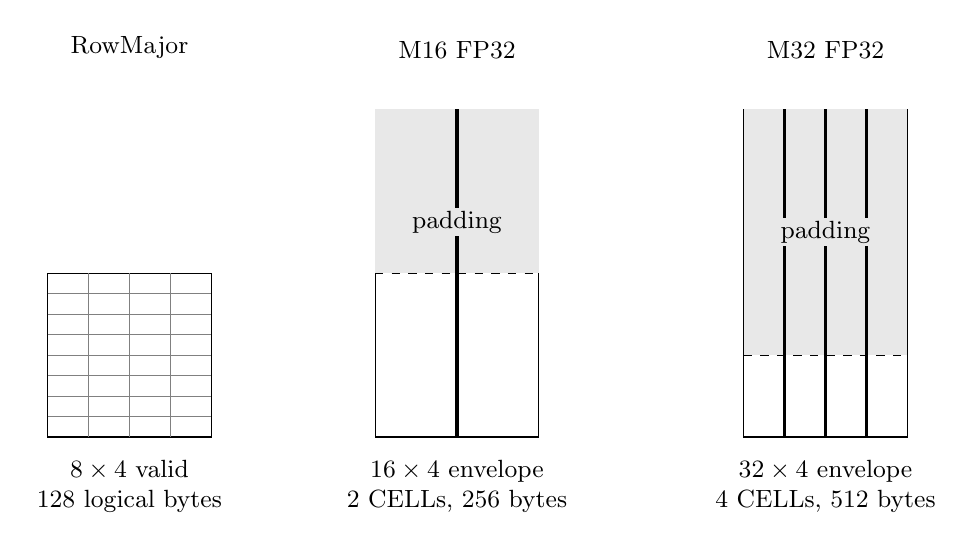
\begin{tikzpicture}[x=0.52cm,y=0.26cm,font=\small]
 \foreach \x/\lab in {0/{RowMajor},8/{M16 FP32},17/{M32 FP32}} {
  \node[anchor=south] at (\x+2,18) {\lab};
 }
 \draw (0,0) rectangle (4,8);
 \foreach \y in {1,...,7}{\draw[gray] (0,\y)--(4,\y);}
 \foreach \x in {1,2,3}{\draw[gray] (\x,0)--(\x,8);}
 \node[align=center] at (2,-2.4) {$8\times4$ valid\\128 logical bytes};
 \draw (8,0) rectangle (12,16);
 \fill[gray!18] (8,8) rectangle (12,16);
 \draw[very thick] (10,0)--(10,16);
 \draw[dashed] (8,8)--(12,8);
 \node[align=center] at (10,-2.4) {$16\times4$ envelope\\2 CELLs, 256 bytes};
 \draw (17,0) rectangle (21,16);
 \fill[gray!18] (17,4) rectangle (21,16);
 \foreach \x in {18,19,20}{\draw[very thick] (\x,0)--(\x,16);}
 \draw[dashed] (17,4)--(21,4);
 \node[align=center] at (19,-2.4) {$32\times4$ envelope\\4 CELLs, 512 bytes};
 \node[align=center,fill=gray!18,inner sep=1pt] at (10,10.5) {padding};
 \node[align=center,fill=gray!18,inner sep=1pt] at (19,10) {padding};
\end{tikzpicture}

\caption{The same eight groups of four FP32 values in three representations. Each diagram has four logical columns; M32 rows are drawn at half the vertical scale. Shading denotes physical rows outside the valid region. CELL divisions describe storage, not execution cycles.}
\label{fig:u005-cells}
\end{figure}

The result also needs an allocation contract. The pinned row-reduction specification creates a new Local destination and preserves its source. The destination has one \emph{valid} column. For CUBE M16/M32 it retains the source's physical column envelope and uses the minimum legal physical row envelope covering the valid rows. In this example, the logical result therefore remains eight FP32 values, but a CUBE destination with four physical columns still carries the 256- or 512-byte envelope above. RowMajor derives its physical rows from the selected destination capacity and one column; its allocation is also not proved to be 32 bytes merely by counting results. A later compaction or layout conversion may reduce storage if the ISA and allocator support it, but that operation and its lifetime must be accounted for. A prefix view alone does not establish that the unused part of an allocation has been returned to the allocator.~\citep{u005-pto-trowsum,u005-pto-reduction-legality}

\subsection{The ordered fold is an architectural constraint}

At PTO revision \texttt{e182c9b}, \texttt{TROWSUM} is selected through the \texttt{TEPL} encoding carrier and dispatched as an SFU block operation. It is not a separate standalone opcode. Its semantic contract is a typed left fold beginning with typed zero, in increasing column order:
\begin{equation}
 a_{g,0}=0_{\tau},\qquad
 a_{g,j+1}=\operatorname{TADD}_{\tau}(a_{g,j},X_{g,j}),\qquad
 y_g=a_{g,K}.
 \label{eq:u005-fold}
\end{equation}
Here $\tau$ is the operation type, including its rounding and status behavior. The contract does not authorize replacing this recurrence by a balanced floating-point tree. Independent groups may run in parallel while each group's observable result and numeric status follow the recurrence. Even then, the actual number of groups processed simultaneously depends on datapaths, ports, issue capacity, and implementation scheduling; it is not given by the semantic definition.~\citep{u005-pto-trowsum}

A concrete FP32 round-to-nearest illustration explains why the distinction matters. For the four inputs
\begin{equation}
 [2^{25},\ 1,\ -2^{25},\ 1],
\end{equation}
the prescribed fold loses the first added $1$ at the large magnitude, cancels the large values, and ends at $1$. A pairing that first forms $(2^{25}+1)$ and $(-2^{25}+1)$ rounds both pairs to the large signed powers of two and then obtains $0$. The real-arithmetic sum is $2$. This example is a derived numerical illustration, not a benchmark or a claim about another architecture's default reduction mapping. It shows that ``four inputs, two tree levels'' is not a legal optimization merely because it looks like the same mathematical sum.

The initial addition from typed zero is also part of the defined operation. An implementation may simplify it only when it preserves the type's full observable semantics, including exceptional inputs and status. Integer addition in the pinned contract retains element-width bits at each step; no separate wider accumulator is implied. The input carrier can be an equal-width non-packed view where the contract permits, but a view is an interpretation, not an arithmetic conversion. An FP32 matrix accumulator elsewhere in the architecture does not grant FP32 accumulation to a typed FP16 reduction.

There is a further implementation boundary. The pinned legality list admits types whose floating fold helper does not yet define an element result: the public reader guidance identifies TF32, HF32, E4M3, and E5M2 as reaching an incomplete \texttt{ScalarFPBinaryProfile} path. The article therefore does not present FP8 sum as an established complete executable capability. A type name in the legal-type list and a complete numeric implementation are separate evidence. Resolving this gap requires a specified arithmetic profile and validation, not merely adding an instruction name to a table.~\citep{u005-pto-trowsum}

\subsection{Masks, padding, and incomplete groups}

The current reduction contract includes every coordinate in the valid source rectangle. It rejects the generic Local CUBE ExecutionMask, including mask state supplied directly to the model. This is different from the shared PE mask: an all-zero PE mask is a strict no-op at a coarser participation boundary. The PE mask cannot be substituted for arbitrary per-element reduction participation. These rules prevent an implementation from silently treating a general element mask as a supported ragged reduction.~\citep{u005-pto-reduction-legality}

For a flat length $N$ grouped by four, let $G=\lfloor N/4\rfloor$ and $r=N\bmod4$. The $G$ complete groups have shape $[G,4]$. If $r\ne0$, the final group requires separately defined handling: a smaller legal shape, a distinct scalar/vector path, or explicitly materialized identity values under a numerical contract that permits them. Padding \emph{outside} a valid rectangle does not make those elements participants in the reduction. Conversely, extending the valid rectangle and filling it with zeros changes which typed operations occur. Such a change must preserve the required rounding, signed-zero, NaN, and status behavior rather than relying only on a real-arithmetic identity.

The same issue appears in masked softmax. An inactive logit is often represented by a suitable negative infinity before the maximum and exponential stages, but the behavior of an all-masked row must still be chosen. A sum's identity, a maximum's identity, and the output policy for an empty normalization are different decisions. The current nonzero-dimension requirement also means an empty Tile cannot be assumed to encode an empty reduction with a convenient default result. Compiler-generated tails have to respect these legality and result rules.

\subsection{Four PE local reductions and a shared Tile Register merge}
\label{sec:u005-four-pe}

Four processing elements (PEs) can cooperate in two fundamentally different ways. First, each PE can own complete, independent reduction groups. For the eight groups of four in Equation~\ref{eq:u005-four}, assign groups $0,1$ to PE~0, groups $2,3$ to PE~1, and so on. Each PE produces two final group results. No cross-PE combine is needed to compute those eight answers, although distributing inputs and handing results to their eventual consumers can still require movement and synchronization. This mapping exposes parallelism \emph{between} groups without changing the prescribed arithmetic \emph{within} a group.

Second, the four PEs can own disjoint subsets of the \emph{same} global group. If one row has $K$ inputs and PE~$p$ owns the subset $I_p$, then a local reduction produces a partial $s_p$. Under a numerical contract permitting this decomposition, the logical construction is
\begin{equation}
 s_p=\operatorname{reduce}_{j\in I_p}(X_j),\qquad
 y=\operatorname{merge}(s_0,s_1,s_2,s_3),
 \quad \biguplus_{p=0}^{3} I_p=\{0,\ldots,K-1\}.
 \label{eq:u005-pe-partials}
\end{equation}
Four local answers are not four final answers to that one global reduction. A consumer needing $y$ must obtain the contribution from every required participant. Different ownership of the same logical axis changes the communication requirement, even when the local reduction instruction is unchanged.

The proposed target architecture makes a shared Tile Register available as a handoff location for PE-produced values. Its intended role here is to let a larger reduction be partitioned across PEs, locally compress each partition, publish those smaller partials, and read them for a final merge. This is a \emph{target-design discussion}; the present source inspection does not demonstrate a particular physical shared-register topology, port count, merge datapath, throughput, or synchronization implementation. ``Shared Tile Register'' names the intended visible handoff resource, not a measured zero-latency or infinitely multiported structure.

\begin{figure}[tb]
\centering
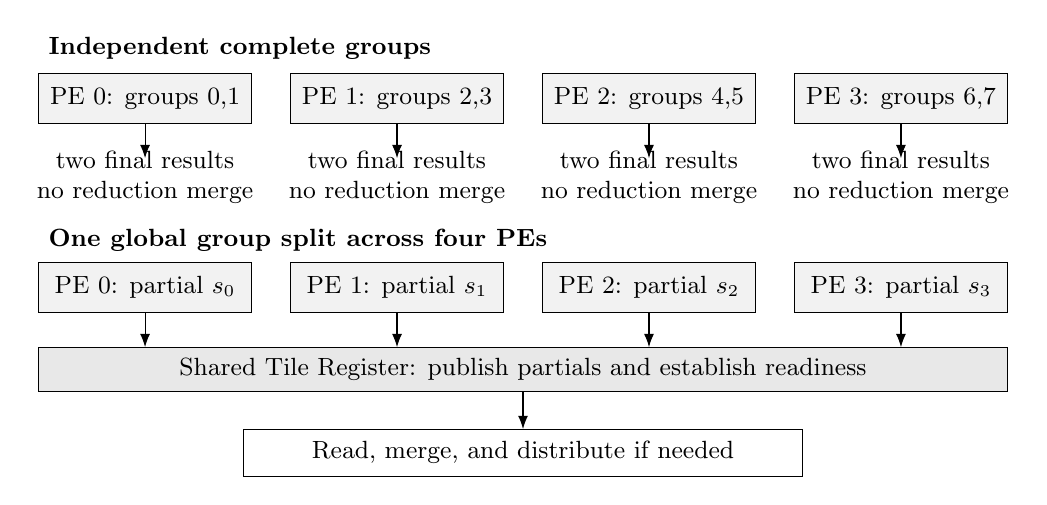
\begin{tikzpicture}[x=1cm,y=0.8cm,font=\small,>=Latex]
 \node[anchor=west,font=\small\bfseries] at (0,5.4) {Independent complete groups};
 \foreach \x/\p/\g in {0/0/{0,1},3.2/1/{2,3},6.4/2/{4,5},9.6/3/{6,7}} {
  \draw[fill=gray!10] (\x,4.2) rectangle (\x+2.7,5);
  \node[align=center] at (\x+1.35,4.6) {PE \p: groups \g};
  \draw[->] (\x+1.35,4.2)--(\x+1.35,3.65);
  \node[align=center] at (\x+1.35,3.35) {two final results\\no reduction merge};
 }
 \node[anchor=west,font=\small\bfseries] at (0,2.35) {One global group split across four PEs};
 \foreach \x/\p in {0/0,3.2/1,6.4/2,9.6/3} {
  \draw[fill=gray!10] (\x,1.2) rectangle (\x+2.7,2);
  \node at (\x+1.35,1.6) {PE \p: partial $s_{\p}$};
  \draw[->] (\x+1.35,1.2)--(\x+1.35,0.65);
 }
 \draw[fill=gray!18] (0,-0.05) rectangle (12.3,0.65);
 \node at (6.15,0.3) {Shared Tile Register: publish partials and establish readiness};
 \draw[->] (6.15,-0.05)--(6.15,-0.65);
 \draw (2.6,-1.4) rectangle (9.7,-0.65);
 \node at (6.15,-1.025) {Read, merge, and distribute if needed};
\end{tikzpicture}

\caption{Two logical ownership choices for four PEs. The upper path assigns complete groups locally. The lower path needs a cross-PE merge and a numerical contract permitting its partial-reduction order. Input/output movement still exists in the upper case. This target-design diagram specifies neither physical topology nor timing.}
\label{fig:u005-pe-ownership}
\end{figure}

For a long row, local compression can substantially reduce the logical data handed to the merge relative to forwarding every input. For example, four partitions of 256 FP32 values contain 4096 input bytes in total; four FP32 partials contain 16 logical bytes. That arithmetic is only a payload comparison. If all four partials are written to shared storage and read once by one merger, the handoff accounts for 16 logical write bytes and 16 logical read bytes, before physical transfer granularity, padding, metadata, contention, result storage, or broadcast. Keeping the merger's own partial local could avoid one of those shared write/read pairs. The actual traffic and allocation follow the supported Tile and register organization. The earlier CUBE-envelope example is a reminder that 16 logical bytes do not establish a 16-byte physical allocation or shared transfer. Conversely, splitting a four-element group across four PEs leaves one value per PE, so there is no local reduction compression before the exchange; distributing whole short groups may be the more useful mapping.

A shared handoff needs an explicit producer--consumer protocol. Each partial requires a unique group and generation identity, storage ownership, and a rule establishing when its payload is visible. The merge must depend on all required partials, or incrementally combine arrivals while still waiting for the last required contribution before publishing the final result. Reusing a partial's slot must wait until every relevant reader is finished. If multiple PEs subsequently normalize their own input partitions, the final sum, maximum, or reciprocal must also be made available to each consumer. A single merger's completion does not by itself broadcast the result or release every participant's state.

Hardware readiness tracking could enforce these dependencies without software executing a full barrier after every local step. Such an implementation still performs synchronization in the architectural sense: it prevents a dependent read from preceding publication and prevents reuse from preceding consumption. A shared register does not remove those causal edges. It moves their enforcement into a particular combination of descriptors, ready bits, dependency joins, arbitration, and possibly software events. The scope and granularity of publication must also be defined; a reader cannot assume that observing one ready CELL makes all other partials ready.

The cost ledger therefore includes shared-register read/write bandwidth, bank and port conflicts, arbitration, temporary partial storage, readiness joins, the merge engine, and result distribution. If $r_p$ is the time at which PE~$p$'s required partial becomes visible, then publication of a final result using every contribution cannot precede $\max_p r_p$. A merge can overlap earlier work and consume partials as they arrive, but it cannot manufacture the missing slow participant's value. Load imbalance, a delayed input, or contention on one PE can therefore dominate the final dependency. If all four PEs need the statistic, broadcast or repeated reads add another resource demand whose cost depends on the actual fabric.

\paragraph{Exact fold versus distributed reassociation.}
Equation~\ref{eq:u005-pe-partials} is not automatically a legal implementation of the current floating-point \texttt{TROWSUM}. The pinned contract in Equation~\ref{eq:u005-fold} begins from zero and visits columns in order. Independently folding each partition from zero and then merging its sum generally changes rounding and status compared with that global recurrence, even if the partitions are contiguous and the final merge visits them in column order. Passing the running accumulator to the next contiguous partition and continuing the ordered additions can preserve the arithmetic recurrence, using a separately supported sequence or implementation mechanism. Current \texttt{TROWSUM} exposes no seed-accumulator operand. Full instruction equivalence must also preserve complete-source preflight, accumulated numeric status, and atomic publication of the result and descriptor. An ordered handoff therefore does not by itself establish an implementation of the full instruction contract, and it does not provide four independent arithmetic folds of one row. A different summary representation or exact accumulator would require its own proof of equivalence, not an assumption that four rounded partial sums suffice.

Independent complete groups remain parallelizable under the current contract. A reassociative distributed sum needs separate, explicit numerical permission, including accumulation type, rounding, exceptional-value/status behavior, and the required reproducibility or error tolerance. Maximum also needs specified NaN, signed-zero, and tie behavior before exchanging arbitrary partial maxima is treated as interchangeable with an ordered reference. Hardware visibility and arithmetic equivalence are separate requirements: a perfectly synchronized merge can still compute the wrong specified floating-point result.

\paragraph{When to prefer each mapping.}
Keeping complete short groups local is a strong default candidate when there are enough independent groups, balanced work, and a suitable input layout. It avoids a cross-PE reduction merge and can reduce shared-port and readiness pressure. It is not a universal winner: there may be too few groups, an excessively long row, uneven ownership, or a producer/consumer layout that makes a shared handoff advantageous. A cross-PE partition can enlarge the usable parallel work and spread storage or local arithmetic over several PEs when its numerical contract permits it. Its benefit must exceed partial publication, read/merge, waiting, and distribution costs. The comparison should report both the saved local work per PE and the newly required shared work, rather than presenting ``four local reductions'' as either automatically complete or automatically faster.

\subsection{NVIDIA GPU ownership can remove or introduce exchanges}

In a common SIMT mapping, a thread combines its register-local values, then participating lanes exchange partial results with warp shuffles. Multiple warps usually need another coordinated stage, often using shared memory, and a reduction split over multiple thread blocks needs a further merge protocol. This hierarchy is a mapping choice rather than an intrinsic number of stages for every tensor. XLA's GPU emitter documentation explicitly describes shuffle and shared-memory lowering for reductions.~\citep{u005-xla-emitters}

API and ISA generation matter. The CUDA 13.0.3 warp \texttt{\_\_reduce\_*\_sync} signatures cover integer arithmetic and bitwise functions; floating-point cooperative reduction examples can use shuffle-based lowering. That observation must not be generalized into the absence of all floating-point warp reduction instructions. PTX 8.7 documents FP32 minimum and maximum forms of \texttt{redux.sync} for \texttt{sm\_100a}, including defined NaN behavior, but does not provide an FP32 addition form in that instruction family. Thus a softmax maximum and sum need not use the same mechanism.~\citep{u005-cuda-reduce,u005-ptx-redux}

A contrasting example is FlashAttention-4's data-center Blackwell mapping: a thread can receive a complete 128-element score-tile row from tensor memory, making that row's reduction register-local. This removes a cross-thread exchange for the cited mapping while increasing or retaining other obligations: register capacity, tensor-memory movement, buffering, and pipeline coordination. Its treatment of exponential work also changes the balance between special-function service and ordinary arithmetic/register use. It is evidence of algorithm--layout co-design, not proof that Blackwell reductions are universally local to one thread.~\citep{u005-flash4}

Many-short-row cases can pack several independent groups within a warp; long-row cases can distribute work more broadly. The compiler must choose participation masks and merge structure consistent with the numerical requirement. Triton's fused-softmax tutorial illustrates a row-resident strategy with power-of-two padding and explicit attention to register/shared-memory occupancy. Keeping a row on chip can avoid rereading it while reducing the number of resident programs. The appropriate comparison to a direct Tile operation therefore includes the best row-ownership mapping that satisfies the same contract, rather than a deliberately communication-heavy baseline.~\citep{u005-triton-softmax}

\paragraph{Pinned CUDA examples expose ownership transitions.}
The \texttt{csrc/flash\_attn/src} path at FlashAttention repository commit \texttt{94e22c90} illustrates a local-then-exchange implementation. Its \texttt{thread\_reduce\_} loops over each thread's fragment; \texttt{reduce\_max} then calls \texttt{Allreduce<4>}. The helper in \texttt{utils.h} performs XOR shuffle exchanges with offsets 2 and 1, with a combine at each step. These exchanges form logical four-thread groups inside a warp; the helper uses a full-warp participation mask. This is local register arithmetic plus scoped lane exchange, not a shared-memory write/read or a CTA-wide barrier. The source and participation requirements must be respected rather than treating every occurrence of \texttt{sync} as the same operation.~\citep{u005-fa-softmax-pinned,u005-fa-utils-pinned}

The same softmax path keeps row-sum partials local while updating the running statistics and performs \texttt{quad\_allreduce\_} in \texttt{normalize\_softmax\_lse} when the combined denominator is needed. Delaying that cross-thread sum avoids repeating an unnecessary exchange at every online update. This is a specific code path and revision; it does not describe every FlashAttention version, the separately discussed Hopper path, or every Blackwell/CuTe kernel.~\citep{u005-fa-softmax-pinned}

OneFlow commit \texttt{25c8978c} makes a second boundary explicit. Its \texttt{WarpAllReduce} uses an XOR-shuffle loop. Its \texttt{BlockAllReduce} instead calls CUB with shared temporary storage, has thread zero write a shared result, executes \texttt{\_\_syncthreads()}, and returns the shared broadcast value. The caller's broadcast/barrier is visible independently of CUB's internal algorithm. Counting local accumulation, shuffles, shared accesses, and barriers separately is more informative than labeling both variants ``many synchronizations.''~\citep{u005-oneflow-softmax-pinned}

Separately, CCCL commit \texttt{dc7fcbdc}'s deterministic warp-reduction specialization writes one aggregate per warp into shared storage, executes a block barrier, and lets thread zero combine the warp aggregates. That specialization also contains an alternative non-deterministic addition path; it is not a universal description of all CUB reductions. Nor does citing this current CCCL file prove that the pinned OneFlow build uses that same dependency revision or specialization. These examples establish scoped mechanisms, not matched latency measurements.~\citep{u005-cub-warpreduce-pinned}

\subsection{Compare shared handoff resources at matching scopes}
\label{sec:u005-shared-scope}

GPU shared memory and the proposed shared Tile Register can both serve as on-chip producer--consumer handoff storage. That functional similarity is useful, but their names do not establish the same physical memory tier, topology, access width, port organization, or visibility contract. In particular, ``register'' does not by itself prove lower latency or higher effective bandwidth than GPU shared memory. Conversely, a shared-memory-based reduction does not inherently imply an off-chip round trip.

There are several GPU comparison scopes. Register-local arithmetic has no inter-thread exchange for that combine. A warp shuffle exchanges values among participating lanes without staging the value through shared memory. A CTA shared-memory merge crosses warp ownership on the CTA's SM and requires the relevant visibility/coordination protocol. A cross-SM merge is a wider problem: ordinary CTA shared memory is not arbitrary chip-wide shared storage. Supported compute-capability-9.0 clusters provide distributed shared-memory access within a bounded co-scheduled cluster, with existence, synchronization, and lifetime requirements; other inter-block decompositions need an appropriate global-memory or multi-kernel protocol. The four-PE target must be compared with the scope those PEs actually occupy, rather than charging every GPU alternative for a cross-SM merge while treating the target's four PEs as adjacent local participants.~\citep{u005-cuda-shared-scope}

The potential advantage of the shared Tile Register is conditional. If its actual implementation provides high effective bandwidth, short producer-to-consumer latency, and dependency-aware consumption of ready partial Tiles, it may avoid a more distant storage path or conservative whole-workgroup waiting in a particular baseline. The baseline might already use nearby shared memory, shuffles, or asynchronous barriers, so the avoided work must be identified rather than assumed. The comparison needs equal logical grouping, numerical semantics, data placement, and result-consumer scope.

Measure or model effective read/write bandwidth under the real access pattern, latency from production to dependent use, bank conflicts, simultaneous read/write ports, arbitration, and contention with matrix/vector traffic. Include readiness publication and joins, slow-participant delay, output broadcast or repeated reads, physical allocation granularity, and the state required for safe reuse. An apparent reduction in explicit barrier instructions is a programming/control-placement result until those costs and the resulting latency are established. Shared storage and dependency hardware can make a handoff cheaper without making synchronization disappear.

\subsection{Ascend composes reduction scopes on a vector path}

Ascend C exposes pairwise, block, repeat, and larger reduction interfaces. Local buffer placement, masks, source strides, destination strides, and pipeline dependencies determine how those operations compose. A documented CANN 8.0 example for 256 FP32 inputs compares repeated whole reductions, repeated block reductions, and a block reduction followed by a whole reduction. The relevant architectural lesson is that a larger reduction primitive is not necessarily the best first stage. Intermediate storage and barriers remain part of the sequence. Its example timing is not transferred to the Superscalar NPU comparison.~\citep{u005-ascend-composition}

For the documented Atlas A2/A3 \texttt{WholeReduceSum} path in CANN 9.0, operands are half or float with matching source and destination types. A contiguous repeat can cover up to 128 16-bit or 64 32-bit elements. The page specifies a tree-style combination and describes intermediate saturation in its half example. These numerical details differ from an exact typed increasing-column fold. A fair performance study must either require the same numerical semantics on both sides or explicitly quantify the changed accuracy/reproducibility requirement. Product-specific integer or newer-generation extensions must be checked separately.~\citep{u005-ascend-whole}

Ascend's higher-level SoftMax interface exposes the broader sequence: maximum, broadcasting, subtraction, exponentiation, sum, broadcasting, and division, with explicit temporary-space and tiling considerations. ND and blocked NZ representations require different traversal choices. A library can hide this orchestration from application code, but hiding it in a function call does not remove vector work, local-memory demand, or a dependency between the statistics and normalization.~\citep{u005-ascend-softmax}

For a reduction distributed across Ascend cores, local \texttt{BlockReduceSum}/\texttt{WholeReduceSum} composition is only the first stage. Partial publication, cross-core ordering, and merging must be added. The live developer-preview \texttt{SyncAll} documentation shows partial computation written to GM before synchronization and subsequent accumulation. It distinguishes a software signal/polling path from supported hardware synchronization; the pipeline-configurable form is listed for 950 products, not A2/A3. Its residency and event-ownership conditions still apply. This demonstrates a GM/workspace plus synchronization design pattern, not a claim that every Ascend reduction uses software polling or that a barrier itself transfers the partial values.~\citep{u008_ascend_syncall}

\subsection{TPU lowering depends on vector topology and axis}

TPU documentation distinguishes matrix, vector, and scalar units; softmax is vector work in that architectural description. The scaling guide's v5p discussion describes a vector organization with eight sublanes and 128 lanes, with different mechanisms for sublane and cross-lane communication. Consequently, reducing one physical axis is not automatically equivalent to reducing the other. This is a scoped explanatory model, not a universal cycle model for all TPU generations.~\citep{u005-tpu-architecture,u005-tpu-topology}

Pallas TPU exposes block-shape restrictions and local-memory layouts commonly organized around $(8,128)$ units. Its compiler can retain an output window while successive input windows are processed. A reduction can therefore use local vector combines, rolling partial accumulation, layout changes, or a staged algorithm, depending on the shape and retained state. General advice to use 32-bit elementwise computation on narrower inputs is a software choice; it should not be confused with a guarantee about every hardware operation.~\citep{u005-pallas-details}

The cost ledger must distinguish vector ALUs, vector loads/stores, matrix work, transpose, and reduction/permutation resources. XProf exposes such distinctions in its utilization view. Low matrix utilization by itself cannot determine whether the bottleneck is exponentiation, cross-lane reduction, movement, or a preceding scalar dependency. A Superscalar NPU comparison should use the same decomposition rather than treating all non-matrix work as a single interchangeable ``vector'' capacity.~\citep{u005-xprof}

When a TPU reduction crosses physical cores or devices, the two-dimensional VPU axis distinction is no longer the whole problem. Pallas's core-specific interface provides an intra-device remote-copy example with semaphores; the distributed interface exposes asynchronous push DMA with separate send and receive completion. A distributed reduction must compose local partial computation with such movement/merging or an appropriate compiler/runtime collective. These are scoped communication interfaces, not evidence of a shared Tile Register across TPU cores. Buffer lifetimes, topology, semaphore matching, and numerical merge order remain in the comparison.~\citep{u006-pallas-coremap,u006-pallas-distributed}

\subsection{Tenstorrent reduces within an owned tile pipeline}

TT-Metalium's \texttt{reduce\_tile} belongs to the FPU/matrix-engine compute API group. It supports row, column, or scalar results and selected reduction operations. The API consumes source/scaler tiles through circular buffers and produces a result in acquired destination state; result placement and packer-mask setup are explicit. This interface does not imply one generic horizontal SIMD instruction or the same implementation as the separate SFPU/vector path.~\citep{u005-tt-reduce}

The unpack--math--pack pipeline and destination ownership determine how reduction work overlaps with its neighbors. In the documented standard-tile configuration, 32-bit destination storage reduces tile capacity relative to 16-bit storage, and double buffering partitions available state further in exchange for overlap. Destination width alone does not guarantee that every selected compute operation uses full FP32 arithmetic.~\citep{u005-tt-engines}

For a reduction spanning several tiles, the algorithm must combine tile-local partials. If ownership spans cores, that merge additionally involves NoC movement and synchronization. Assigning whole rows to cores can avoid cross-core merging but may expose load imbalance; splitting long rows increases parallel work while adding communication and state. These are general decomposition consequences. The tile API alone establishes neither a distributed reduction guarantee nor complete softmax fusion.

\subsection{Softmax is a chain with retained state}

For one row, stable softmax requires a maximum, subtraction and exponential, sum, and normalization. The intermediate exponentials must be retained or recomputed/read again after the final normalizer is available. Online normalization can merge partial states $(m_a,s_a)$ and $(m_b,s_b)$ using
\begin{align}
 m &= \max(m_a,m_b),\\
 s &= s_a\exp(m_a-m)+s_b\exp(m_b-m).
\end{align}
This identity can reduce passes for the normalizer while adding rescaling arithmetic and partial state. It does not make every output available before the final normalization is known, nor does it guarantee floating-point equality across merge orders.~\citep{u005-online-softmax}

FlashAttention-3 demonstrates a Hopper implementation that overlaps asynchronous matrix multiplication, movement, and softmax work across tiles and warpgroups. The overlap consumes barriers, pipeline stages, registers, and explicit role allocation. It is useful evidence that vector work can sometimes be hidden by matrix work, while the remaining non-matmul service demand still matters. A faster low-precision matrix engine alone does not establish a proportional speedup for maximum, addition, exponential, reciprocal, or movement.~\citep{u005-flash3}

For the Superscalar NPU, a direct row/column operation can carry semantic intent and permit hardware to choose an implementation satisfying it. The current exact-order sum contract restricts that choice more than an associative reduction API. Hardware could interleave independent row folds, pipeline typed additions, or overlap unrelated operations; those are candidate implementations, not proven throughput. A future relaxed-order form would need an explicit numerical permission, separate legality, and testable error/reproducibility guarantees. It cannot be retroactively assumed for \texttt{TROWSUM}.

The architectural benefit condition is therefore precise. A direct Tile reduction helps when it removes software reconstruction or unnecessary communication for a supported shape while preserving required numerics and fitting the live-state budget. Its cost includes source/result port demand, row accumulators, padding/allocation, status aggregation, dependency tracking, and coexistence with exponentials and matrix work. It must be assessed together with U002's lifetimes and U003's layout transformations. The logical reduction result becoming small is only the beginning of that analysis.

\section{U006 Scalar and event orchestration}
\label{sec:u006}

\subsection{A fused workload spans three coordination domains}

Consider a tensor-parallel tile stream: each card produces matrix partials, exchanges them, applies a local vector epilogue or normalization, and publishes data for the next matrix stage. Multiple SoC cores share this work. Fusion brings inter-card communication, local matrix/vector execution, and on-chip multicore synchronization into one dependency graph; removing a launch boundary does not remove their ownership transfers. NVIDIA's NCCL fusion example illustrates reduce-scatter, local RMSNorm, and all-gather. Its current source targets NCCL 2.30 or later and prioritizes teaching clarity rather than maximum performance. It is a concrete protocol example, not an optimized performance ceiling. The surrounding matrix stages here are an illustrative workload, not a claim about that example's implementation.\citep{u006-nccl-fusion}

U001 (Section~\ref{sec:u001}) asks when matrix/vector work becomes ready; U002 (Section~\ref{sec:u002}) owns storage lifetime; U004 (Section~\ref{sec:u004}) owns irregular payload accesses and data atomics; U005 (Section~\ref{sec:u005}) owns reduction execution and numerical contracts. U006 asks who prepares, submits, waits for, and consumes the events connecting those stages. U007 (Section~\ref{sec:u007}) and U008 (Section~\ref{sec:u008}) own precise effects/visibility and bounded-resource progress respectively.

\subsection{Identify the agents before comparing mechanisms}

For each edge, identify five roles: the initiator constructs and submits a request; an executor moves or computes the payload; a waiter checks the relevant completion; a completion consumer updates downstream ownership; and a visibility authority establishes which effects that observation permits. A role may be implemented by the same thread, a different warp/controller, firmware, or hardware. None is determined by the word ``asynchronous.'' A device-side flag is not inherently a host round trip.

For the illustrative tile exchange, compute control prepares a descriptor, a transfer engine or communication role executes it, a receiver observes destination readiness, and a completion service eventually releases the source and returns credit. A multicore handoff may use a different visibility scope from the inter-card transfer. A waiting compute role must not obstruct the executor or the completion consumer that can unblock it. This role ledger is an analytical decomposition, not a prescribed allocation of one hardware thread per role.

\subsection{Four scopes and five milestones}

Within a compute core, scalar control can submit matrix, vector, and copy operations and coordinate local dependencies. Across cores on one chip, communication can use a local NoC, shared global memory, hardware flags, or remote local-memory operations. Across devices, it may use peer loads/stores, remote DMA, NIC queues, or a collective protocol. Host/runtime setup allocates resources, registers memory, constructs communicators, launches work, and tears it down. These scopes have different agents, ordering rules, and failure modes.

For one transfer, at least five milestones should be distinguished:
\begin{enumerate}
 \item The command was accepted or issued
 \item The source is no longer read by the local transfer machinery
 \item The destination payload is visible within the required recipient scope
 \item The consumer has observed the readiness event and consumed the value
 \item The storage and protocol identity can be safely reused
\end{enumerate}
A particular API may combine some milestones, but no combination should be inferred from the word ``complete.'' A flush that permits local source reuse is not necessarily a remote-consumption acknowledgement. An event announcing a byte count is not necessarily an acquire for unrelated memory. Safe tag reuse may additionally require that stale events from an earlier generation cannot match the new owner. These distinctions connect directly to U007's ordering and U008's reclamation obligations.

\begin{figure}[tb]
\centering
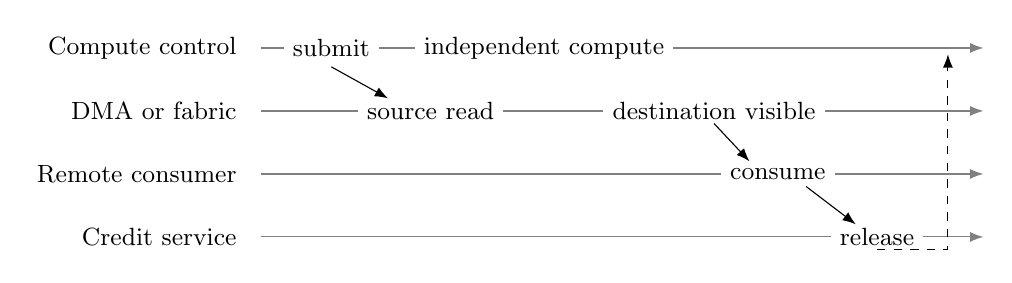
\begin{tikzpicture}[x=0.9cm,y=0.8cm,font=\small,>=Latex]
 \foreach \y/\lab in {3/{Compute control},2/{DMA or fabric},1/{Remote consumer},0/{Credit service}} {
  \node[anchor=east] at (-0.2,\y) {\lab};
  \draw[->,gray] (0,\y)--(10.2,\y);
 }
 \node[fill=white] at (1,3) {submit};
 \node[fill=white] at (4,3) {independent compute};
 \node[fill=white] at (2.4,2) {source read};
 \node[fill=white] at (6.4,2) {destination visible};
 \node[fill=white] at (7.3,1) {consume};
 \node[fill=white] at (8.7,0) {release};
 \draw[->] (1,2.7)--(1.8,2.2);
 \draw[->] (6.4,1.8)--(6.9,1.2);
 \draw[->] (7.7,0.8)--(8.4,0.2);
 \draw[->,dashed] (8.7,-0.2)--(9.7,-0.2)--(9.7,2.9);
\end{tikzpicture}

\caption{A conceptual producer--transfer--consumer protocol. Vertical arrows are required causal edges; horizontal spacing is illustrative and is not a latency measurement. Source reuse, destination readiness, and credit return can require different events and progressing agents.}
\label{fig:u006-events}
\end{figure}

An event that travels through device memory is not automatically a host round trip. PCIe is an interconnect, not an execution agent: a supported peer or NIC path can use PCIe without host software submitting every message. Similarly, an accelerator-side service processor is not the host CPU. A claimed weak-scalar or host-event bottleneck must identify the actual processor, path, and trace rather than generalizing to every NPU.

\subsection{NVIDIA distributes control through roles and device communication APIs}

A warp, a CTA, a thread-block cluster, arbitrary blocks across SMs, and multiple devices are distinct scopes. \texttt{\_\_syncwarp} orders participating warp lanes; \texttt{\_\_syncthreads} is a CTA barrier. Applicable asynchronous-barrier/\texttt{mbarrier} and cluster mechanisms have their own arrival, phase, and visibility rules. They do not turn an ordinary grid barrier into a safe cross-SM synchronization point. Cross-device communication needs the supported transport/library contract.\citep{u006-cuda-scopes}

For on-chip pipelines, Hopper TMA allows a thread to initiate bulk asynchronous movement while other work proceeds. Warp-specialized kernels distribute producer, matrix-consumer, and epilogue work across roles, each with barrier and buffer ownership. CUTLASS contains concrete producer/consumer pipeline implementations. Dedicated roles avoid placing every instruction in one thread's immediate sequence, but consume resident state, registers, barrier phases, and issue opportunities. Thread-block clusters add a bounded cross-block shared-memory scope; they do not make every block in an arbitrary grid simultaneously resident.~\citep{u006-hopper,u006-cutlass}

Across devices, NCCL LSA uses supported peer load/store connectivity; multimem uses supported NVLink SHARP multicast; GIN provides network communication where supported. NIC participation and any proxy path depend on transport and configuration. Its archived 2.28.7 documentation covers symmetric memory windows and device communication contexts, including puts, signals, waits, and flushes. These mechanisms require setup and transport support. In particular, local input reuse after a flush must not be conflated with the remote readiness/signaling obligation. The exact facility must be selected from the topology and library version rather than inferred from the GPU's marketing family.~\citep{u006-nccl}

NVSHMEM provides another division of responsibility. Traditional IBRC uses a CPU proxy; IBGDA permits GPU construction of NIC work-queue entries, doorbell updates, and completion handling in GPU memory. CPU-assisted variants place parts of the work differently. Device initiation therefore names a control capability, not one universal data path. The vendor's performance guidance explicitly discusses the cost of GPU WQE construction, contention when issuers share queue pairs, and the resource/fence cost of more queues. Moving submission to the GPU can expose parallel issuing but does not establish a lower single-message latency in every configuration.~\citep{u006-nvshmem-ibgda,u006-nvshmem-performance}

For a fused kernel, account for scheduler and register residency, shared memory, flags and barrier state, atomic and load/store ports, submission/completion queues, interconnect/NIC capacity, staging memory, and any proxy work. A waiting warp need not block another ready warp, but still retains registers and other resident resources. The GPU scheduler can select other eligible warps while one waits, but only resident work with available resources can benefit. Synchronizing persistent or collective kernels must follow the library's launch and progress requirements; NVSHMEM documents collective-launch constraints for applicable synchronization/collective use. Ignoring those requirements would compare a correct bounded protocol against an inadmissible one.~\citep{u006-nvshmem-using}

\subsection{Ascend separates pipeline events from communication service}

Ascend C describes scalar control as responsible for scheduling and instruction transmission and advises reducing unnecessary scalar computation and branching. This supports the possibility of scalar pressure in a specified kernel; it does not prove a universal single-thread bottleneck across every Ascend generation. Intra-core \texttt{SetFlag}/\texttt{WaitFlag} operations use pipeline event state, and the receiving pipeline waits for the corresponding event. They are not inherently host or PCIe events. Event identifiers are finite and pairing is part of the programming contract.~\citep{u006-ascend-architecture,u006-ascend-flags}

For supported separate-mode products, cross-core flags provide AIC/AIV synchronization with product- and mode-specific rules. CANN 8.5 documents modes spanning AIC/AIV groups and warns that high-level Matmul internally owns some synchronization resources. A hand-written fused kernel must therefore avoid conflicting with library-owned event IDs. Correctness is a composition problem involving the compiler, library, runtime, and explicit user synchronization, even though the underlying event operation is hardware controlled.~\citep{u006-ascend-crosscore}

For cross-device work, the CANN 9.0 HCCL kernel interface uses an AI Core client and an AI CPU or CCU server, depending on supported hardware and configuration. A Prepare operation supplies the collective description; Commit authorizes execution when dependencies allow it; completion and finalization have separate roles. Descriptor preparation can be moved before compute so that some setup overlaps, while Commit must still respect data readiness. The AI CPU is accelerator-side, so its participation alone does not imply a host-CPU round trip.~\citep{u006-hccl}

The CANN 9.0 AIV task-orchestration example documents another path: readiness flags are written through local-to-global copies, and waits repeatedly copy a GM flag into local storage for scalar comparison. Payload GM-to-GM movement stages through Vector Core local storage. Its example uses before/after rank synchronization and a stable HCCL buffer. A reduce-enabled copy's atomic write belongs to the payload reduction path, distinct from scalar task-queue atomics.\citep{u006-hccl-aiv}

HCCL Host, AICPU/CCU service, and AIV initiation are separate configurations; SDMA, RDMA, Notify, GM flags, and atomic-write capabilities must be attributed to the supported generation and path. The supplied CANN 8.5 alpha002 communication-path page could not be retrieved in this review, so it is retained as an unverified pointer rather than used to establish an SDMA/RDMA/Notify assignment. Neither that gap nor the AIV example supports a universal weak-scalar or host-round-trip claim.

This organization pays for client scalar instructions, server work, handles, queues, communication workspace, and synchronization. Repeated use must maintain the documented Commit/Wait accounting, and finalization cannot race slower participating cores. The useful question is whether preparation, server execution, and completion service stay ahead of the tile stream, not whether the API name contains ``asynchronous.'' A server queue that fills can return pressure to the client, while a client that waits too early can fail to prepare later independent work. Product-specific traces are needed to determine which case limits an actual kernel.

\subsection{TPU uses asynchronous DMA with explicit completion ownership}

Pallas TPU has scalar control and scalar memory for control operands, distinct from vector and matrix computation. Its documented grid execution and memory movement model differs from GPU warp oversubscription: the compiler arranges local-memory transfers and supported multicore partitioning is explicit. Asynchronous engines can advance while scalar control performs other work, but that fact does not create a second independently executing scalar instruction stream.~\citep{u005-pallas-details}

The distributed Pallas interface exposes device-issued asynchronous push DMA within a TPU pod. A descriptor includes distinct send and receive semaphores. Starting the copy can be followed by independent work; the send completion protects local source reuse, while the receive completion protects destination use. The distributed guide demonstrates buffering and pipelining and warns that mismatched waits or counts can cause hangs, crashes, or corruption. These are explicit device-side communication capabilities, so a model that routes every TPU tile exchange through host software would be an unfair baseline.~\citep{u006-pallas-distributed}

The newer core-specific interface exposes physical core meshes, per-core storage/semaphores, and remote-copy examples between cores. It is a distinct interface from older Megacore guidance; their assumptions should not be silently merged. Multiple cores can split control responsibility, but the partition adds ownership, balance, and communication obligations.~\citep{u006-pallas-coremap}

A custom fused Pallas kernel may also obscure opportunities that XLA's higher-level scheduling could exploit. Its local benefit must be compared with the compiler-managed baseline, including asynchronous collective scheduling and neighboring fusion. The retained-state ledger includes VMEM/SMEM, DMA descriptors, semaphore values, in-flight buffers, and ICI contention. An independently progressing DMA protects progress only for work already submitted with adequate destinations and matching completion behavior. It cannot prepare a future descriptor that the stalled scalar program has not issued.

\subsection{Tenstorrent gives data movement dedicated control roles}

The official RISC-V guide's illustrated five-controller Tensix design assigns BRISC/NCRISC to movement and TRISC unpack/math/pack roles to orchestration of compute engines. The RISC-V controllers are not themselves the matrix/vector datapaths. This is a documented design scope, not a controller-count claim for every generation. Reader, compute, and writer work can therefore be expressed as different roles. Circular buffers provide explicit producer/consumer capacity and readiness operations. This division can reduce competition for the compute role's instruction sequence while preserving dependencies through buffer ownership. The reader sequence is CB reserve, asynchronous NoC read, read-completion barrier, then CB push; the consumer waits, computes, and pops. \texttt{cb\_reserve\_back} is explicitly a blocking polling operation and does not advance a CB pointer. The costs include controller state, L1 circular buffers, staging, queues, semaphores, credits, and backpressure.\citep{u006-tt-riscv,u006-tt-cb,u006-tt-roles}

Within a chip, NoC commands, barriers, and remote semaphore updates move data and coordinate consumers. Ordering is scoped by the chosen NoC, command buffers, and virtual channels. Separate NoCs or VCs do not gain a single total order merely because one controller issued commands in source order. A producer must establish the payload-before-signal edge using the appropriate ordered path or completion operation.~\citep{u006-tt-ordering}

Across chips, the older Wormhole/Blackhole Ethernet guide, now explicitly marked outdated in favor of fabric infrastructure, describes staging through Ethernet-core L1 and asynchronous sends. The low-level send primitive does not itself supply the full receiver-completion and source-reuse protocol. Queue-busy handling, acknowledgements or credits, and teardown must be implemented or supplied by a higher-level fabric/collective facility. The guide recommends fabric infrastructure for managing Ethernet cores; comparing only link bandwidth would omit movement between Tensix and Ethernet storage and the resources consumed by fabric workers.~\citep{u006-tt-ethernet}

This approach makes control agents visible and programmable, which can be advantageous for known streaming graphs and explicit placement. More stages, however, mean more protocol state, fill/drain work, and potential recovery boundaries. A dedicated reader can still block on a full circular buffer; a writer can still need credits returned by another participant. Dedicated controllers make independent progress possible but do not prove it under all backpressure conditions.

\subsection{Current contracts and the proposed command-publication path}

PTO snapshot \texttt{e182c9b} provides useful building blocks, not a completed accelerator protocol. \texttt{HL.BFI}, \texttt{BXU}, \texttt{BXS}, and \texttt{HL.CCAT} manipulate scalar fields; constructing a command word is separate from atomically publishing a whole descriptor. The extracted \texttt{BXU/BXS} mnemonics do not have an \texttt{HL.} prefix in that snapshot. The v0 executable \texttt{BSE/BWE/BWI/BWT} semantics record a nonblocking request, operand, and epoch; they do not demonstrate hardware sleep, wakeup arbitration, or a lost-wake proof.\citep{u006-pto-fields,u006-pto-sys}

GQM \texttt{HL.QMT/QPUSH/QPOP} initialize and atomically manipulate a queue of individual 64-bit entries. Push is release and pop acquire by default; \texttt{.r} removes that ordering, and \texttt{.e} notifies only on success. Full or suspended push reports failure; these contracts supply no implicit sleep or fairness. Publishing one entry or pointer does not itself make a multiword descriptor coherent to a device. The memory-ordering owner must establish the descriptor/payload-before-publication edge.\citep{u006-pto-gqm}

Scalar atomics can claim tasks, update queue indices, allocate slots, and count completions. These are orchestration operations, distinct from U004's data atomics. A wider atomic path may support more independent addresses, but a single hot queue counter or ownership word still serializes. Sharding, batching, and hierarchical aggregation are software/design alternatives, with extra state and ordering costs; no speedup is established here.

The proposed target is an explicit chain: construct fields, materialize a descriptor, publish complete ownership, execute at the accelerator, and return identified completion/status/error. Device ordering, cache visibility, admission credits, lost-wake handling, cancellation, and late completion require separate contracts. Historical Linx HAC/private-bus and MSGB documents at \texttt{c7cb8d93} illustrate an earlier message-interface direction using legacy command encoding. They are historical context, not evidence that this future chain is implemented or that its current ABI is settled.\citep{u006-linx-hac,u006-linx-msgb}

\subsection{Fusion changes the rate at which control must be performed}

A fused pipeline can remove intermediate launches and unnecessary memory boundaries while creating more frequent interactions between its internal stages. For every tile, an implementation may calculate addresses, prepare descriptors, reserve storage, submit work, publish readiness, handle a completion, and return credits. These operations are useful work in the control path. If they cannot keep up, independent compute and communication engines can wait even though their payload bandwidth is not saturated.

Consider a steady stream of tiles. Let $c$ denote the required scalar/control instructions per tile, $\mu_s$ the sustainable control service rate in instructions per unit time, $t_m$ matrix service time per tile, $t_v$ vector service time, and $t_d$ movement/communication service time. Under ideal overlap with independent resources, a necessary lower bound on the steady-state initiation interval is
\begin{equation}
 I\ \geq\ \max\left(t_m,t_v,t_d,\frac{c}{\mu_s}\right).
 \label{eq:u006-control}
\end{equation}
If two stages use the same non-overlappable resource, their demand must be combined rather than placed in separate terms of the maximum. A dependency chain or insufficient buffering can raise $I$ further. The equation is an analytical accounting device, not a model calibrated to a particular processor.

Smaller tiles can reduce the delay before a consumer sees useful output, but they generally increase the number of control episodes per useful byte. If a tile carries $b$ bytes and requires $e$ events, the event density is $e/b$. Reducing $b$ while retaining the same protocol can increase this density even when the arithmetic work scales proportionally. The crossover depends on scalar issue capacity, event hardware, message aggregation, buffer size, and the independence available to cover latency. ``Fuse more'' is therefore incomplete guidance unless the control path is included.

\subsection{Provision outstanding work from submission through completion drain}

Core issue queues are only the first admission point. An end-to-end outstanding budget must cover NoC credits, receiver slots, reply capacity, and completion drain, as well as request queues and live descriptors. For rate $\lambda$ and average occupied lifetime $L$, $\lambda L$ is an analytical average occupancy requirement under stable conditions, not a sufficient capacity guarantee under bursts, failures, or delayed peers. Capacity at one stage cannot compensate for a full receiver or stalled reply path. Completion traffic must retain a route and service opportunity when compute or submission is blocked.

The component ledger therefore includes scalar issue/atomic/load-store ports, contexts and register state, descriptor construction, queues and arbiters, local staging/buffers, NoC/NIC credits, receiver/reply state, and completion/status processing. Shared resources combine demand; hot addresses remain serialized. Measure fill, steady state, and drain separately rather than counting only accepted requests as progress.

\subsection{Conditional Superscalar NPU benefits}

Scalar issue width and SMT context count are tunable resource parameters. Wider issue can overlap independent field/address work if dependencies and ports allow it; multiple contexts can separate submission, local compute orchestration, and completion service if arbitration and retained state permit progress. A default of four STIDs or a decode width of two/four/six is not an issue-width result or proof that four contexts suffice. Proposed coroutine scheduling is a software organization for moving to other ready work; it does not create independent hardware progress by itself.

Compiler-planned roles and late waits can combine with hardware-managed local dependencies and a bounded independent completion path. Event/DMA offload can reduce repeated instruction work for already-described operations. These are proposed conditional benefits: enough independent work and end-to-end capacity must exist, ownership/visibility must be correct, and saved waiting must exceed added control/state/interference. Current queue/request semantics, historical interfaces, and analytical occupancy reasoning establish neither a measured SSNPU advantage nor a complete cross-card protocol. U007 and U008 supply the corresponding precision and progress boundaries.

\subsection{What a matched evaluation must observe}

A credible experiment would record the control instructions and events per tile, time spent preparing and issuing work, outstanding descriptors, queue-full stalls, live buffers, and the agent responsible for each wait. It would separately measure fill, steady state, and drain across tile sizes and rank counts. Register or local-memory growth from added roles must be included, as must host/runtime setup when it is not amortized. No fixed orchestration penalty or cross-platform speedup is inferred here.

The decision rule is whether the chosen control organization lets every necessary event arrive soon enough without excessive state or interference. Fusion removes some boundaries and brings others inside a kernel. The architecture succeeds when it makes those internal boundaries inexpensive, precise, and live under the actual resource limits, rather than merely invisible in source code.

Evidence classification in this chapter is explicit: pinned PTO contracts are normative/current; versioned vendor mechanisms are documented within their scope; Linx HAC/MSGB and the outdated low-level Ethernet guide are historical; the command-publication chain and coroutine organization are proposed; occupancy and component-cost reasoning are inferred analytical accounting. Any integration candidate beyond those contracts remains unverified. No measured SSNPU performance or PPA result is supplied.

\section{U007 Precise faults and ordering across asynchronous engines}
\label{sec:u007}

The useful correctness contract for a fused accelerator must say which effects have occurred, which state can be inspected, and which operations can safely be repeated. A matrix operation can finish after a younger scalar instruction, a vector consumer can start before an unrelated transfer finishes, and a remote receiver can consume an output before the sending host observes completion. These are ordinary consequences of overlap. The difficulty arises when a programmer, debugger, or recovery mechanism treats all these events as one undifferentiated notion of completion. The design objective is therefore to preserve necessary causal edges while giving faults a well-defined attribution and recovery boundary. Serializing every engine makes some executions easier to inspect, but discards much of the overlap that U001 and U006 seek to expose.

Consider a distributed tile pipeline. A local matrix stage produces an intermediate, a vector stage transforms it, a communication engine transfers the result, and a remote stage consumes it. The algorithm determines the producer--consumer relation. The ISA or device API determines how that relation becomes an ordering or completion guarantee. The compiler translates the relation into commands and synchronization; the runtime determines submission, participant identity, and failure handling; hardware tracks the resulting state. A missing edge can originate in any of these layers. Conversely, moving an edge from explicit software to dependency-tracking hardware changes its implementation and ownership, without eliminating the edge or the resources needed to enforce it.

\subsection{Four contracts that must not be conflated}

A \emph{precisely attributed fault} identifies the operation that caused a failure, possibly including an instruction address, tile identifier, engine, memory address, and source location. A \emph{precise recoverable state} is stronger: the saved architectural state corresponds to a specified instruction boundary, and execution can resume according to a stated restart rule. The classical precise-interrupt definition is based on a sequential architectural boundary; in-order completion is one implementation, while retained versions and recovery structures permit execution and completion to be less restricted \citep{u007_smith_pleszkun}. For a modern accelerator, the definition must identify its recovery domain and the status of pending effects outside that domain.

A \emph{memory-order contract} specifies permissible observations and synchronization relationships, including address spaces, atomicity, participants, and scopes. It does not necessarily impose one total order over the machine. A \emph{completion and ownership contract} specifies when an operation has reached a named milestone and when a resource may change owners. An operation can have finished reading its source while its destination remains unavailable to a consumer. A receiver can have received a tile while still retaining it for computation. These cases require different events even when one implementation happens to report several of them together.

\begin{table}[tbp]
\centering
\small
\begin{tabularx}{\linewidth}{@{}p{0.21\linewidth}XX@{}}
\toprule
Contract & Question answered & What does not follow automatically \\
\midrule
Fault attribution & Which operation caused this error? & Registers and memory form a restartable snapshot \\
Precise local state & At which specified boundary can this domain resume? & Remote consumers can undo escaped effects \\
Memory ordering & Which observations must precede which others, for which observers? & All transfers are complete or all participants have arrived \\
Completion & Which operation milestone has been reached? & Every consumer has stopped using the payload \\
Ownership release & Who may overwrite or reclaim this storage now? & The containing pool can be deallocated \\
Trace or replay & Which events were recorded or can be reproduced? & Every race or unrecorded schedule has been covered \\
\bottomrule
\end{tabularx}
\caption{Correctness and observability contracts answer different questions. Each guarantee needs an explicit scope.}
\label{tab:u007-contracts}
\end{table}

An asynchronous error adds a further distinction between the \emph{cause} and the \emph{reporting point}. For example, the CUDA driver documents that synchronization-related calls can report errors from earlier asynchronous launches \citep{u007_cuda_context}. The call returning an error is thus a useful observation boundary, but need not be the offending operation. A debugger likewise needs to distinguish the faulting program counter from the later counter at which an engine stopped. Even a correct fault address cannot reconstruct a tensor already overwritten by younger work.

\subsection{A publication and reuse example}

Let device A produce tile $X_e$ for epoch $e$ in source slot $S$, and let device B receive it into slot $D$. Define events $W_e$ for the final producer write, $I_e$ for transfer issue, $S_e$ for source-read completion, $D_e$ for destination arrival, $P_e$ for publication of readiness, $C_e$ for the end of the consumer's reads, and $A_e$ for acknowledgment that the destination slot can be reused. The following is an abstract protocol requirement, not a vendor instruction sequence:
\begin{align}
 W_e &\prec I_e, & S_e &\prec \operatorname{overwrite}(S), \label{eq:u007-source}\\
 D_e &\prec P_e \prec \operatorname{read}_B(D), &
 C_e &\prec A_e \prec \operatorname{overwrite}_{e+1}(D). \label{eq:u007-dest}
\end{align}
The symbol $\prec$ means an established causal relation under the selected API and memory model. It is not a claim that an arbitrary local fence implements that relation. Publication may need a release/acquire pair, a DMA completion event, an ordered data-and-signal primitive, or more than one of these. The choice depends on the path by which payload and signal reach the consumer.

Suppose the payload travels on one channel and the ready flag on another. Source-code issue order alone is insufficient unless the selected interface orders those channels. B can observe the flag while reading old or partially updated data. Adding a local fence with a scope that excludes B also fails to establish the required edge. In another failure, A reuses $S$ after merely enqueuing the transfer, so the transfer observes a mixture of two epochs. In a third, A correctly waits for delivery but overwrites $D$ before B finishes consuming it. All three are synchronization errors, but they require different repairs: publication ordering, source completion, and destination ownership respectively.

The protocol need not place a global barrier after every tile. A finite set of destination slots can carry distinct epochs, and the sender can advance whenever it owns a free slot and the required completion state. This retains overlap while making the ownership proof explicit. It also reveals why an epoch or generation identifier is useful: a delayed readiness signal for $e$ must not satisfy a wait for $e+1$. Whether a finite identifier can wrap safely depends on the maximum lifetime of outstanding work and the reuse protocol; a wide counter by itself is not a proof.

A communication API may permit source release before the receiver can consume the destination. Pallas remote DMA exposes separate send and receive waits \citep{u007_pallas_distributed}. Tenstorrent's documented on-chip NoC path similarly distinguishes source-flush completion from destination-arrival completion, while its low-level Ethernet path requires a higher-level acknowledgment protocol for comparable guarantees \citep{u007_tt_ethernet}. These mechanisms instantiate different subsets of the abstract events. They should not be collapsed into one generic barrier in a performance diagram.

\subsection{What a local precise-state design must establish}

For a proposed superscalar NPU, take a local architectural instruction sequence $i_0,i_1,\ldots$ and a retirement frontier $k$. A precise exception at $i_k$ requires a state consistent with the specified boundary before that instruction, subject to its documented fault or partial-completion semantics. All older architectural effects must be represented as completed effects or irrevocably committed pending effects according to the contract. Younger effects must be invisible to observers covered by the rollback guarantee. This is a local sequential boundary, not a promise of globally sequentially consistent memory.

A sufficient construction for \emph{faults detected before commit} can be stated with four invariants. First, committed register and tile mappings identify the versions produced by the retired prefix. Second, speculative versions cannot overwrite the only recoverable version of any live architectural value. Third, externally observable side effects are either withheld until their issuing operation is irrevocable or covered by an explicitly specified transactional recovery protocol. Fourth, every outstanding operation retains a generation-valid identity and reports either successful completion or a fault before it becomes eligible to commit. An implementation may enforce these invariants with renaming, checkpoints, result buffers, ordered publication, or a mixture; a ROB is only one part of the construction.

The corresponding argument is inductive. Initially the committed mappings and effects represent the empty prefix. A successful retirement updates them only after the instruction's required results and fault checks are complete, preserving the next prefix. If the oldest faulting instruction reaches the frontier, younger speculative versions are discarded and the previous committed mappings restored. The side-effect invariant prevents discarded instructions from leaving an observable effect inside the promised recovery domain. The identity invariant prevents a delayed response from an old execution from updating a recycled destination. Under these assumptions the recovered state represents the last retired prefix. This argument is conditional on the invariants; their names in a design document are not evidence that every engine enforces them.

Several difficult cases remain visible rather than disappearing into the proof. An in-place tensor update needs an undo method or a preflight rule strong enough to prevent partial modification on the covered fault classes. A long matrix instruction that permits partial architectural completion needs a restart cursor or another precise description of which suboperations are committed. An error discovered after retirement, such as a later asynchronous integrity failure, falls outside the before-commit proof unless the architecture retains the necessary recovery information. Cancellation must establish whether a command has actually stopped, whether its responses can still arrive, and which resources it continues to own. Silently treating ``cancel requested'' as ``all effects canceled'' breaks both state recovery and allocation safety.

Remote publication is the hardest boundary. Suppose a younger instruction on A sends a value that B uses to update its own state, and an older instruction on A subsequently faults. Restoring A's rename map cannot undo B's computation. A design must therefore delay the send's visibility until the relevant local boundary is irrevocable, define the send as an explicit non-rollback boundary, or use a distributed protocol that can coordinate recovery. Delaying publication can retain a large output and add retirement-head blocking. A distributed protocol adds epochs, acknowledgment, duplicate suppression or idempotency, and agreement about what has committed. None follows from an instruction carrying a ROB identifier.

\subsection{NVIDIA GPU ownership and tooling}

PTX provides an explicit scoped memory model for the documented $\texttt{sm\_70}$-and-later scope, with specified exclusions, rather than treating asynchronous execution as unrestricted memory behavior. Its proxy rules also matter when asynchronous engines and ordinary accesses interact; ordinary ordering and asynchronous completion are separate obligations \citep{u007_ptx}. At the runtime layer, streams and events let software establish dependencies without synchronizing the entire host and device. A stream wait can defer downstream work while unrelated work remains eligible \citep{u007_cuda_async}.

NVIDIA's debugging facilities expose useful but different contracts. Compute Sanitizer distinguishes precisely attributed instrumented access errors from less precisely attributed hardware exceptions. Its race and synchronization checking have documented coverage; they do not prove arbitrary global or distributed code race-free, and error termination does not roll back earlier outputs \citep{u007_compute_sanitizer}. CUDA-GDB documents fault-origin reporting separately from the later stopping PC, and offers autostep to improve localization in selected regions \citep{u007_cuda_gdb}.

The algorithm or library chooses synchronization scope and buffer ownership; the compiler preserves the relevant source semantics; runtime events connect launches; device mechanisms implement the specified ordering and completion. The resulting control inventory includes per-thread or warp execution state, readiness and dependency tracking, barrier state, asynchronous command identities, and debug instrumentation where enabled. The exact circuit topology need not be known to recognize these functions. Conversely, profiler or debugger features do not establish a CPU-style ROB implementation or universal instruction restart.

The benefit condition is concrete: explicit scopes and event dependencies are valuable when independent work exists outside the required dependency cone. Broad waits may be simpler to audit but retain less overlap; finer dependencies require more precise ownership reasoning and state. Instrumentation can improve attribution while perturbing the schedule that exposed the original error. A fair comparison therefore records production semantics, diagnostic mode, and recovery scope separately rather than comparing an instrumented GPU with an uninstrumented proposal.

\subsection{Ascend compiler and framework synchronization}

Ascend C describes scalar issue to asynchronous vector, matrix, and movement pipelines. In the cited CANN 8.5 interface, cross-pipeline flags connect producer completion to consumer execution, while pipeline barriers constrain a selected pipeline. The compiler and framework insert substantial synchronization, including documented Vector and Cube responsibilities; manual cases remain when the automatic analysis or movement-address assumptions are insufficient. The documentation distinguishes portable TQueSync interfaces from hardware-sensitive ISASI forms \citep{u007_ascend_sync}. Consequently, describing Ascend kernels as universally hand-scheduled barriers would overstate the author burden, while treating framework synchronization as an unrestricted proof would hide its assumptions.

msSanitizer documents memory-hazard checking across supported memory and pipeline combinations, with source-context reporting and release-dependent coverage \citep{u007_ascend_sanitizer}. msDebug supports hardware debugging and core analysis, but explicitly warns that execution can continue for several instructions before an exception is reported: saved registers and memory can be inaccurate even when the PC is corrected \citep{u007_ascend_debug}. This is direct evidence that accurate attribution and coherent recoverable state must be assessed separately, without dismissing the diagnostic value of the tools.

Responsibility is distributed across algorithmic staging, tensor-lifetime analysis, framework-owned flags, runtime completion, and hardware pipelines. The design costs include event state and ownership, local buffer lifetimes, waits inserted conservatively when aliases are uncertain, and the resources used by diagnostic instrumentation. Automation is especially valuable when a kernel stays inside the framework's analyzable ownership model. Custom aliasing, unusual pipeline interactions, or library composition can shift obligations back to the author. The cited term ``committed'' in a pipeline-barrier description should be interpreted under that API, not promoted to an unprovided architectural retirement guarantee.

\subsection{TPU compiler dependencies and low-level Pallas control}

OpenXLA uses tokens to express side-effect dependencies, including joins through \texttt{AfterAll} \citep{u007_xla_tokens}. This is a compiler-IR contract. It does not reveal a complete physical TPU memory model or imply that independent physical engines execute sequentially. Pallas makes a lower-level boundary visible: software pipelining coordinates asynchronous units and buffer lifetimes, trading additional storage for earlier movement and later waits \citep{u007_pallas_pipeline}. The compiler can absorb regular scheduling work when the kernel supplies the necessary dependence and lifetime information.

For distributed kernels, the programmer still needs correctly matched transfers, synchronization counts, slot reuse, and participant identity. Pallas documents separate completion milestones and failure modes for mismatched synchronization \citep{u007_pallas_distributed}. Its debugging guide describes interpreted race detection and compiler-pass dumps \citep{u007_pallas_debug}. A simulation can explore memory and synchronization behavior and a compiler dump can expose a missing edge; neither is evidence of the exact silicon execution that failed, nor proof that all permitted schedules were checked.

The costs arise in both generated and explicit control: semaphore state, buffer versions, scheduling metadata, and the retained payload needed while communication overlaps computation. A compiler can simplify the normal programmer's contract without removing these functions. The proposed superscalar alternative should therefore be compared against the compiler's optimized schedule and actual debug facilities, not against an imagined TPU with no synchronization or visibility. Public evidence reviewed here leaves general instruction-level precise restart unspecified; that is an evidence boundary, not a claim that a particular hidden microarchitecture cannot support recovery.

\subsection{Tenstorrent explicit ownership and scoped communication}

TT-Metalium documents that writes on the same NoC and virtual channel follow program order; using different NoCs or virtual channels does not automatically preserve that order \citep{u007_tt_ordering}. Reader, compute, and writer roles must connect movement completion to circular-buffer publication and consumption. A queue-ready condition says that the producer has published data under the queue contract, so the producer must establish the required payload completion first. The receiver's eventual slot release is another event.

Watcher provides kernel identities, per-controller waypoints, and selected address or bounds checks. Its current hardware-exception PC/cause reporting is explicitly Quasar-specific \citep{u007_tt_watcher}; that capability cannot be silently attributed to Wormhole or Blackhole. The experimental NoC Debug Dump reports selected missing barriers and outstanding writes, while warning that timing can hide faults and tracing adds overhead \citep{u007_tt_noc_debug}. Waypoints and traces are valuable localization aids, but do not constitute a coherent global checkpoint.

The ownership split is particularly visible: kernels and libraries arrange roles, channels, buffer handoff, and completion; controllers and engines advance the specified operations; runtime or fabric software manages broader program lifetime. The benefit is that communication and compute control can be separated and overlapped with explicit storage boundaries. The price includes controller instructions, buffer and semaphore state, trace capacity, and the need to compose several local protocols correctly. This is a different distribution of control from a superscalar instruction window, not an absence of control logic.

\subsection{The proposed superscalar NPU and the full cost of precision}

The supplied project inspection records ROB control, renamed identities, completion and non-flush gates in a timing model, with a separate typed bring-up path containing its own identity and recovery contracts. These observations motivate a local precise-state design; they do not establish one integrated, verified implementation. In particular, neither a model component nor a source-level retirement routine proves that every tensor update, local transfer, atomic, and remote effect obeys the invariants above.

The proposal's strongest plausible advantage is a simpler local programming and debugging boundary: source-level operations could retain stable provenance while dependency tracking permits safe internal overlap. That advantage applies where the architecture can identify dependencies and control publication, and where the cost of retaining recoverable state is acceptable. It becomes weaker for irrevocable remote effects, uncertain memory aliases, very large in-place updates, or long-latency operations that block the retirement frontier. These cases need explicit semantics, rather than a blanket claim that out-of-order hardware makes asynchronous code easy to debug.

A useful provenance chain maps source operation to compiler IR, emitted instruction or command, dynamic epoch, engine issue, completion, retirement, and fault. Many-to-one fusion and one-to-many lowering must remain representable. Trace records should identify lost records and distinguish per-engine order from cross-engine timestamp order. Otherwise a visually tidy timeline can suggest causal edges that the machine never guaranteed. Deterministic replay, if desired, needs a separate account of external inputs and scheduling decisions that influence execution.

The cost ledger must include exception records, tags and generations, committed and speculative mappings, retained payload versions, output-publication buffers when needed, and arbitration on recovery paths. Retaining an old tile can occupy an existing physical pool rather than require a new full-tile copy; the important quantity is unavailable capacity over time, not only copy count. Let $b_v$ be the bytes occupied by version $v$ and $[a_v,r_v)$ its retention interval. The analytical occupancy integral
\begin{equation}
 \mathcal{R}=\sum_v b_v(r_v-a_v)
\end{equation}
helps compare recovery schemes with different lifetimes, while peak occupancy determines capacity feasibility. Neither quantity alone predicts energy, area, or throughput. Metadata width, array ports, selection logic, checkpoint traffic, and the critical timing path require implementation evidence.

The appropriate correctness result is therefore a stated recovery domain and a proof or verification argument for every effect that can cross it. The appropriate performance result is reduced unnecessary ordering or debugging work after counting the storage and control that preserve that domain. Local retirement, scoped memory order, asynchronous completion, and distributed recovery remain separate contracts whose composition must be designed deliberately.

\section{U008 Forward progress under finite resource constraints}
\label{sec:u008}

Correct dependency tracking does not ensure that a dependent operation will ever execute. A producer can own a valid tag and a correctly counted destination reference while waiting indefinitely for storage; the operation that would release that storage can itself be unable to enter the machine. Backpressure preserves a capacity limit by stopping admission or movement, but can also propagate a wait to the only useful releaser. The architectural question is therefore specific: what may admitted work retain while blocked, who can remove the blocking condition, and why can that agent obtain every resource it needs?

This question spans the layers already encountered in U002 and U006. The algorithm creates dependencies and determines whether a consumer can run without another input. The ISA and API define waits, completion, ownership, and permitted execution scopes. The compiler chooses live ranges, buffering, and stage order. The runtime admits kernels, assigns participants, and manages communication epochs. Hardware allocates finite entries and arbitrates service. Static scheduling, dynamic readiness selection, and explicit dataflow distribute these tasks differently; each still needs a capacity and progress argument.

\subsection{State the property before selecting a mechanism}

A safety property forbids an invalid event, such as overwriting a live tile or accepting a stale completion. A liveness property requires a useful event eventually to occur. The difference matters because a machine can protect every live value by waiting forever. Four progress outcomes should be kept distinct:
\begin{description}[style=nextline]
\item[Deadlock freedom] No reachable unfinished state contains a permanently blocked set under the stated environment and execution assumptions. A closed circular resource wait is one cause of deadlock; waiting for a signal that no participant will ever produce is another.
\item[System-wide useful progress] Useful operations continue to complete while work remains. This can hold while one particular operation is indefinitely bypassed.
\item[Starvation freedom] Every admitted operation within the promised scope eventually receives the service required to complete, assuming its external prerequisites satisfy the contract.
\item[Bounded completion latency] Completion occurs within a specified bound. Eventual service alone supplies no finite numerical upper bound.
\end{description}
A long stall can be legal if its producer or external service eventually responds. Livelock is different again: retries, cancellations, or state changes continue, but no useful result completes. A timeout detects an exceeded waiting interval; without additional evidence it does not identify which of these conditions occurred.

Progress is relative to a scope and model. A resident thread, a workgroup, a complete kernel, a device, and a distributed collective need different assumptions. Research on GPU workgroup progress formalizes how termination depends on the selected relative-progress model \citep{u008_sorensen}. That distinction is useful here; historical experiments on particular devices are not certification of every later scheduler. Similarly, an eventual-service assumption for the network excludes a permanently failed peer. A fault-tolerant claim must say how such a failure changes the goal from normal completion to detected failure, resource recovery, or job restart.

\subsection{A capacity ledger and a resource-wait graph}

For each finite pool $r$, partition its capacity into occupied storage $O_r$, reservations for future occupancy $V_r$, and unassigned capacity $F_r$:
\begin{equation}
 C_r=O_r+V_r+F_r,\qquad O_r,V_r,F_r\geq 0.
 \label{eq:u008-capacity}
\end{equation}
These categories are disjoint. An arriving payload converts an existing reservation into occupancy; it must not consume a second credit for the same slot. If in-flight data has no destination reservation, some other documented buffer or backpressure rule must be able to retain it. ``The load has not bound its final tile'' says nothing by itself about where the returned bytes wait. Logical identities, payload slots, transfer descriptors, completion records, and execution contexts are separate pools even when a particular implementation couples their allocation.

A useful wait-for graph has operations and resource instances, not merely data dependencies. An edge from an operation to a resource means that the operation needs that resource to advance. An edge from a resource to an operation identifies its holder or the operation that must run to release it. Signals can be represented through their producing operations. For multi-instance pools, a cycle in a coarse graph is only a warning: a free instance, a preemptible holder, or another release route can break it. A deadlock claim needs a reachable state, the actual capacity counts, and evidence that every relevant route is blocked.

Acyclic algorithmic dataflow does not eliminate these resource edges. Two independent subgraphs can contend for a shared command pool and turn an otherwise straightforward schedule into hold-and-wait. Conversely, cyclic algorithmic dataflow can be live with the correct initial tokens and capacity. The relevant graph must therefore include the initial state, allocation order, release conditions, and any independent completion mechanism. Counting only matrix and vector operations omits the control work on which their continued issue depends.

\subsection{A worked saturation example}
\label{sec:u008-example}

The following small machine is an illustrative construction, not a report of a defect in any vendor product or the supplied project model. It has two physical payload slots $P_0,P_1$, two normal command entries $Q_0,Q_1$, and two return-buffer slots $R_0,R_1$. At the chosen point, $P_0$ and $P_1$ contain completed outputs $x$ and $y$. Both are safe to publish and have no remaining local consumers. Each output can release its payload slot after a drain transfer has finished reading it. A drain requires a normal command entry in the baseline machine.

Now admit two independent loads, $L_0$ and $L_1$. Each retains its command entry until its returned value has been bound into a physical payload slot. Their returns $z_0,z_1$ have arrived and occupy $R_0,R_1$. The loads wait for free payload slots; draining $x$ or $y$ waits for a command entry. The allocation policy allowed these two loads to consume the last normal command entries before admitting either drain. No cancellation, spill, preemption, or alternate command path exists in this hypothetical baseline.

\begin{table}[tbp]
\centering
\small
\begin{tabularx}{\linewidth}{@{}p{0.15\linewidth}p{0.15\linewidth}XX@{}}
\toprule
Pool & Capacity & Occupancy at the blocked state & Condition needed for release \\
\midrule
Payload $P$ & 2 tiles & Completed outputs $x,y$ & A drain obtains a command entry and finishes reading \\
Commands $Q$ & 2 entries & Loads $L_0,L_1$ & A return binds into a free payload slot \\
Returns $R$ & 2 tiles & Returned values $z_0,z_1$ & The corresponding value binds into $P$ \\
\bottomrule
\end{tabularx}
\caption{Illustrative saturated state. The example's release rules are assumptions, not inferred hardware policies.}
\label{tab:u008-blocked}
\end{table}

There is a concrete circular wait:
\begin{equation}
 \text{loads hold }Q
 \;\longrightarrow\;
 \text{loads need }P
 \;\longrightarrow\;
 \text{drains must release }P
 \;\longrightarrow\;
 \text{drains need }Q.
 \label{eq:u008-cycle}
\end{equation}
The return buffers are full but are not the essential cycle in this construction. Increasing their depth alone cannot make a command entry or payload slot available. Fair selection among the loads also cannot help: both are ineligible for the missing capacity. Nor does a larger instruction window help if every newly visible drain must acquire the same exhausted $Q$ pool. The failure is a resource-admission and release-path problem, despite the absence of a data dependency from $x$ or $y$ to either new load.

Several repairs are possible. Admission could keep one normal command entry available for drains. The scheduler could issue the drains before allowing the loads to occupy all command entries. Command identity could be decoupled from the resource retained during return binding, provided some other completion-tracking capacity is guaranteed. A completed output could be spilled through an independently provisioned path. Each repair changes a particular hold-and-wait edge and has a cost. Merely adding a retry loop changes no edge.

\subsection{An escape path with a conditional progress argument}

For a more explicit repair, add one escape command entry $Q_E$ and one escape completion record $E_E$, unavailable to ordinary loads. An escape drain can read an already publishable payload directly, transmit it to a sink with prearranged capacity, and release its payload after source-read completion. Its descriptor, arbitration, completion notification, and capacity return do not require $Q$ or $R$. The drain may use a shared data path only if it is guaranteed eventual service there. A reserved descriptor is ineffective if the request subsequently joins a blocked normal completion queue.

Temporarily stop admitting new work at saturation, and give the escape path a finite batch of already admitted work to retire. For this example, assume all four payloads $x,y,z_0,z_1$ are terminal outputs, each safely drainable once resident. An allowed sequence is shown in Table~\ref{tab:u008-drain}. A dash denotes a free slot; entries show the state after each macrostep, rather than a cycle-accurate timing trace.
\begin{table}[tbp]
\centering
\small
\begin{tabularx}{\linewidth}{@{}p{0.43\linewidth}XXX@{}}
\toprule
Completed macrostep & Payload $P$ & Normal $Q$ & Returns $R$ \\
\midrule
Initial blocked state & $x,y$ & $L_0,L_1$ & $z_0,z_1$ \\
Escape-drain $x$ & $-,y$ & $L_0,L_1$ & $z_0,z_1$ \\
Bind $z_0$ and finish $L_0$ & $z_0,y$ & $-,L_1$ & $-,z_1$ \\
Escape-drain $y$ & $z_0,-$ & $-,L_1$ & $-,z_1$ \\
Bind $z_1$ and finish $L_1$ & $z_0,z_1$ & $-,-$ & $-,-$ \\
Drain $z_0$ and $z_1$ & $-,-$ & $-,-$ & $-,-$ \\
\bottomrule
\end{tabularx}
\caption{One feasible drain sequence for the explicitly bounded example. The existence of this sequence is supplemented by service and scheduling assumptions in the text.}
\label{tab:u008-drain}
\end{table}

A feasible sequence alone proves only reachability of completion. To obtain a liveness argument, specify the controller and its service assumptions. It retains a selected drain until that drain completes; the selected drain's remaining local and external steps receive eventual service. When a return and a free payload slot coexist, binding receives eventual service, and its bookkeeping can release $Q$ and $R$ without allocating from either pool. There is no new admission or rollback during this finite drain phase. These assumptions rule out indefinite bypass as well as circular capacity waits in the stated scope.

Let $b$ count the two admitted loads whose binding remains unfinished, and let $d$ count the four output drains that remain unfinished, including outputs not yet bound. Define
\begin{equation}
 \Phi=b+d.
 \label{eq:u008-ranking}
\end{equation}
Every completed bind reduces $b$; every completed drain reduces $d$; neither step increases the other count because all admitted outputs were counted initially. If $P$ contains a value, an escape drain is available under the example's terminal-output assumption. If $P$ is empty and $b>0$, a returned value can bind. The selected macrostep eventually finishes under the service assumptions, so $\Phi$ strictly decreases after finite intervals until it reaches zero. Intermediate transfer states need not decrease $\Phi$; their eventual completion is an explicit premise. This establishes finite-batch local draining and reclamation for the example, without asserting a cycle bound. If a drain releases its source before destination arrival, remote delivery remains an outstanding obligation: its transport records and destination reservation must survive local reclamation. Proving receiver completion requires including that obligation and its eventual-service assumption in the progress measure or in a separate composed argument.

The argument does not cover an arbitrary computation graph. A resident tile might still be speculative, needed by an unfinished consumer, or impossible to drain without another local operand. A remote sink might need the same saturated network path to return a credit. Those cases require a different invariant or a larger protected resource set. Reserving one entry is sufficient only after proving that one entry plus its complete dependency chain can advance. The reserve also consumes capacity that ordinary work could otherwise use, and a drain phase can reduce normal overlap. Its benefit is saturation robustness under this explicit contract.

\subsection{NVIDIA GPU residency and collective ordering}

CUDA's ordinary blocks must support independent execution, including sequential scheduling. A resident block therefore cannot assume that an arbitrary nonresident block will execute while it waits. Cooperative grid synchronization uses an occupancy-bounded cooperative launch; compute-capability-9.0 clusters add a co-scheduled group whose scope is the cluster. Independent Thread Scheduling does not supply arbitrary inter-block progress, and Programmatic Dependent Launch explicitly treats concurrency as opportunistic rather than a correctness guarantee \citep{u008_cuda_guide}.

This divides ownership cleanly. The algorithm must use a legal synchronization structure. Compiler-selected register and shared-memory footprints influence residency. The runtime validates or arranges the supported launch, and hardware schedules within that contract. A change in resource footprint can invalidate an informal argument based on a previous occupancy estimate. Phase-separated kernels can avoid an in-kernel global wait, at the cost of another boundary; cooperative admission can keep required participants resident, at the cost of limiting the admitted grid. Neither mechanism proves a user lock protocol or mismatched barrier correct.

Distributed execution adds ordering among communication operations. NCCL 2.26 introduced optional implicit ordering between communicators on a device, while requiring consistent host launch order across devices; its documented error handling includes asynchronous-error polling and communicator abort/recreation \citep{u008_nccl}. These are software-contract mechanisms for a bounded class of interactions. They cannot be replaced by an assumption that every queued GPU kernel or collective will run concurrently. The control costs include launch and participant state, resident execution resources, events, and recovery coordination; exact undocumented scheduler fairness is not inferred.

\subsection{Ascend lifetimes and core admission}

The live Ascend C developer-preview documentation describes a TPipe--TQue model that separates stage handoff from storage reuse. Enqueue/dequeue operations connect producer and consumer stages, while tensor allocation and release govern slots in local pools \citep{u008_ascend_tque}. The compiler and framework can implement regular stage protocols, but their composition must still fit the finite buffer and synchronization resources. A released tensor slot is useful only if the stage that performs the release can execute.

CANN 9.0 documents an additional admission boundary. Normal scheduling may launch an operator in parts as physical cores become available. The \texttt{\_\_schedmode\_\_(1)} qualifier enables batch mode, which waits for the required physical cores before launching the kernel. The documentation recommends this mode for the specified concurrent inter-core-synchronizing scenario to avoid partial operators waiting on one another's unavailable cores. The illustrated cost is lost overlap between those operators \citep{u008_ascend_batch}. The live SyncAll developer-preview API also constrains logical block count relative to the physical cores available to the operator \citep{u008_ascend_syncall}.

This is a useful example of preventing a residency cycle before it forms. It is scoped to supported products and the documented scheduling mode, not a claim that every Ascend task is gang scheduled. Algorithm authors and libraries choose participants and pair synchronization; the compiler preserves stage dependencies; runtime admission secures the cohort; pipeline hardware advances events and movement. Local queue correctness and cohort admission solve different parts of the problem. Additional buffering may absorb stage imbalance but consumes local memory and lengthens live intervals. Batch admission may simplify an inter-core proof while reducing overlap, and still needs a fair policy among waiting kernels if starvation freedom is promised.

\subsection{TPU compiler lifetimes and distributed capacity}

Pallas exposes asynchronous unit coordination through compiler-managed pipelines, buffers, and semaphores. Multibuffering consumes local capacity to let movement run ahead of computation \citep{u007_pallas_pipeline}. The Pallas asynchronous-operation design also makes lifetime preservation across split start/done operations explicit, including synchronization resources that remain live until completion \citep{u008_pallas_async}. A compiler can reason about these intervals only when outstanding work remains represented after its start operation has issued.

Across devices, Pallas documents capacity semaphores or additional slots to restrict producer run-ahead, unmatched-wait failure modes, and barrier-identity discipline across invocations \citep{u007_pallas_distributed}. Capacity control and transfer completion serve different purposes. A received payload can still occupy a slot until its consumer releases it. An old invocation's signal must not satisfy a later invocation's rendezvous merely because the same semaphore resource is reused.

The algorithm supplies matching communication and the consumer's dependency structure. The compiler manages visible local schedules and lifetimes; kernel or library code supplies the distributed protocol; runtime invocation identity and hardware service complete the contract. The benefit of static planning is strongest when shapes and communication structure permit a dependable capacity schedule. Dynamic latency still requires waits or spare slots, and a local schedule does not establish remote service. Costs include VMEM or other scratch occupancy, semaphore and epoch state, scalar control instructions, and startup/drain work. More slots permit skew at a memory cost; stronger per-step synchronization restricts skew by sacrificing overlap. Neither choice is universally preferable.

\subsection{Tenstorrent queue and fabric composition}

TT-Metalium circular buffers expose bounded producer/consumer ownership. The producer checks capacity before writing and publishing; the consumer waits for available pages and releases them after use. In particular, \texttt{cb\_reserve\_back} is documented as a blocking capacity poll that does not advance a pointer, so its name should not be read as an atomic allocator spanning arbitrary producers \citep{u008_tt_cb,u008_tt_reserve,u008_tt_pop}. Correct page accounting prevents overwrite; it does not prove that a downstream actor can be scheduled or acquire its other inputs.

The Wormhole Ethernet guide describes higher-level flow control using acknowledgments and receiver buffer availability, together with startup and teardown coordination for asynchronously executing programs \citep{u007_tt_ethernet}. The dependency chain includes the controller processing credits and the lifetime of the remote program, not only the payload link. A queue protocol that is live while both programs run can fail to compose with teardown if one side stops before servicing the other's final acknowledgment.

Algorithm and placement determine graph topology, initial tokens, and buffer depth. Kernels or fabric libraries arrange producer/consumer protocols; controllers and communication engines provide execution and movement; runtime setup establishes participating programs and resources. This explicit decomposition helps expose where capacity is held. It also makes control work visible in RISC instructions, circular-buffer counters, semaphores, routing buffers, and acknowledgments. Increasing L1 buffering can absorb imbalance but cannot repair an unmatched receive or a closed wait involving controllers. The relevant benefit condition is a graph and placement whose local queues and communication lifetimes compose under finite capacity, not an assumption that every dataflow graph is inherently live.

\subsection{The proposed superscalar NPU needs a completion proof}

The supplied timing-model inspection distinguishes logical tile identity from physical payload binding. A conditional local-load path can defer binding until returned data is ready, while ordinary issue-time binding remains. Guarded release checks consumers, a non-flush boundary, aliases, and physical references. These are useful mechanisms for shortening some holding intervals, with a clearly limited evidence scope. They do not establish that every instruction can bind late, every partial read frees storage, or every admitted operation eventually completes.

Late binding removes an early claim on one pool but extends dependence on another. The unbound operation still needs logical identity, request tracking, return retention, and a future binding opportunity. If it holds an entry needed by a storage-releasing operation, the hypothetical cycle above explains the form of proof required, without asserting that the reviewed model contains that cycle. A dynamic scheduler can exploit a ready releaser only if it is represented in the reachable window, passes ordering gates, and can acquire the resources on its completion path.

Generation tags and reference accounting primarily establish safety. They prevent a stale response from modifying a recycled entry or an old consumer from decrementing a new value's count. A liveness argument additionally needs eventual servicing of bind requests, completion records, reference decrements, and releases. A precise-state design from U007 can prolong retention because an old version remains recoverable until retirement; a progress repair must not free that version merely to break a wait. Recovery and liveness therefore constrain the same physical storage, rather than being independent features added after scheduling.

One defensible design method is to enumerate, for each admission class, the resources held before issue, during execution, while awaiting return, and through architectural commitment. Then identify at least one legal route from every admitted unfinished state to useful completion or reclamation, and establish that the permitted scheduler cannot avoid such progress indefinitely. The route can be a compiler-certified phase, a resource-order discipline, reserved completion capacity, or an escape protocol. Its proof must include ordinary and conditional late-binding paths, not only the favorable path drawn in an example. If a retry or rollback is involved, repeated attempts need an argument that excludes unbounded recovery churn.

\subsection{Fairness and cost complete the contract}

Weak fairness requires eventual service for an action that remains continuously enabled. It does not generally protect an action that repeatedly becomes eligible and loses a short-lived opportunity. Stronger fairness assumptions or a bounded-overtaking policy may be needed when binding and arbitration interact. Aging an instruction can affect selection among eligible candidates, but does not allocate a missing buffer or make a nonresident participant runnable. Admission fairness, issue fairness, network service, and completion/reclamation fairness must be stated at their own boundaries.

A numerical latency claim requires stronger premises still. In a finite batch, if every selected macrostep has a bounded service time and the scheduler bounds the number of overtaking operations, a completion-time bound can be constructed from those limits. Replacing either bound by ``eventually'' leaves only eventual completion. In an open system with unbounded arrivals, even a deadlock-free queue needs admission or service-rate assumptions before a finite waiting bound is meaningful. These are mathematical conditions for a claim, not performance measurements of the architectures discussed here.

The common ledger includes reserved-but-idle capacity, queue and credit state, generation checks, arbitration and aging, completion bandwidth, extra buffer residence, and the overlap lost to phase or gang admission. A global acquisition order can remove circular hold-and-wait but constrain scheduling freedom. Releasing before waiting can remove an edge but require reconstructible state and safe reacquisition. Escape capacity can secure a drain path but reduces ordinary usable capacity. Timeouts and aborts can bound fault detection or trigger recovery only when recovery itself has a runnable path and a defined effect on outstanding traffic.

A credible forward-progress claim therefore names its participants, capacities, initial state, failure assumptions, release paths, and fairness obligations. Public GPU, Ascend, TPU, and Tenstorrent interfaces provide concrete mechanisms for parts of this contract. The superscalar proposal changes resource lifetimes and selection opportunities, which may reduce stalls under suitable conditions. It must meet the same standard: admitted work retains a complete, safely reclaiming path that the specified execution policy will eventually service. No architecture-wide or distributed guarantee follows solely from backpressure, additional buffering, a ROB, or a larger instruction window.

\section{Cross problem synthesis and an evaluation agenda}
\label{sec:synthesis}

\subsection{The common object is a value with obligations}

Across the eight problems, a useful unit of reasoning is a value together with its obligations: the operations that produce it, the valid coordinates and numerical meaning, its consumers, its storage owner, and the events that permit reuse. A value is not exhausted by its payload bytes. A delayed memory request can require identity and return capacity before compute storage is bound. A reduced result can contain only a few logical elements while retaining a larger physical envelope. An asynchronously transmitted value can be locally complete yet still relevant to remote consumption or recovery.

A compiler can establish many obligations statically when control and access patterns are predictable. A kernel can encode them explicitly in thread roles, barriers, and buffers. Hardware can track them dynamically when readiness and resource availability vary. The architectural decision is where each obligation is most economically enforced while preserving a coherent contract between layers. This view avoids treating static scheduling, SIMT, dataflow, and superscalar issue as mutually exclusive answers to every part of an operator.

\subsection{Where the proposed mechanisms can help}

Fine-grained readiness is useful when consumers need independently valid subsets and when work released early has an available execution path. It provides little benefit if the next stage requires a global statistic, if every candidate waits on the same resource, or if the reduced coordination interval is smaller than the new bookkeeping cost. Partial readiness therefore needs both a semantic proof and a resource feasibility argument.

Late binding is useful when request latency occupies a substantial part of the early-reservation lifetime and when returns can be safely buffered or assigned capacity on arrival. It cannot eliminate the live payload needed by a consumer. Savings in final compute storage must be offset against return buffering, metadata, fragmentation, arbitration, and progress reserves. A system with a full return queue and no way to reclaim final storage can be worse than one with conservative early reservation.

Typed Tiles can carry the logical shape, representation, and axis of an operation, allowing software to avoid repeatedly rebuilding that meaning from individual lanes. This is an expressiveness and compilation benefit when the chosen operations are supported. It does not remove conversion, scale handling, packing, invalid tails, or numerical constraints. An exact-order reduction deliberately limits reassociation; an indexed atomic with returned old values deliberately limits aggregation. Such constraints must remain visible when judging potential throughput.

Independent scalar or event progress is useful when control work would otherwise serialize compute and communication. It must be paired with finite-resource allocation and fair shared-resource access. A second controller that waits on the same exhausted pool may add state without opening a drain path. Event offload that cannot recover or distinguish generations can trade a visible software protocol for a harder-to-debug hardware failure.

\subsection{A common experimental design}

A future matched evaluation should begin with a workload family rather than one favorable kernel. The dense family should vary independent output count, matrix tile shape, reduction length, dtype, layout, and the proportion of non-matrix work. The irregular family should vary index locality, duplicate rate, fan-out, sparse degree distribution, returned-value use, and supported atomic order. The distributed family should vary tile/message size, rank count, topology, imbalance, and service delays. These variables expose the conditions in the eight arguments without assuming that one mechanism is always active or useful.

The required outputs include end-to-end latency, steady-state throughput, and separate fill/drain contributions. Storage should be reported as an occupancy trace or live-interval distribution, not only a peak allocation constant. Movement should be counted at each interface, including conversion and staging. Control accounting should include dynamic instructions, events, descriptors, tag and queue state, selection/arbitration work, and time blocked for capacity. Physical comparisons require matched implementation technology and clock/area/power methodology; source-level counts cannot substitute for that evidence.

The numerical baseline must be explicit. Compare exact-order folds with exact-order folds, or state that reassociation is permitted and quantify the resulting error/reproducibility requirement. Distinguish FP32 storage from FP32 arithmetic and accumulation. The memory baseline must likewise be explicit: atomics, acquire/release scopes, result publication, safe reuse, and error recovery must satisfy equivalent obligations. A kernel that omits required synchronization is not a faster implementation of the same contract.

Ablations should disable or constrain one proposed mechanism at a time while keeping the rest of the workload and machine budget meaningful. Examples include whole-Tile versus partial readiness, early versus delayed binding with the same total storage accounting, fixed versus dynamic issue within the same finite window, and shared versus independent completion service. Enlarging every queue to conceal a liveness flaw is not a valid ablation. Each configuration must first satisfy safety and the progress property it claims.

\subsection{Correctness and progress before performance conclusions}

A useful validation hierarchy starts with executable instruction semantics and boundary cases, then compiler lowering and complete operator equivalence, then finite-capacity protocol testing, and finally performance/physical implementation. It includes shape and mask legality, type/encoding errors, collisions and old values, deterministic publication, buffer-generation reuse, exceptional numeric status, and memory-order litmus tests. Progress validation must include capacity saturation, delayed peers, simultaneous returns, fairness, cancellation, and the release path itself.

A passing finite test set is evidence, not a general proof. Where a design makes a broad claim such as deadlock freedom, it needs explicit invariants and environmental assumptions, with model checking or another defensible proof method for the relevant state space. Starvation freedom additionally needs an arbitration argument. A bounded latency claim requires bounded service and arrival assumptions, not just the absence of deadlock. These distinctions should survive into performance reports rather than being hidden in a single ``works'' label.

This article has not executed those model tests, compiler tests, benchmarks, or synthesis flows. It provides the contracts and questions that make such work interpretable. Approximate utilization or improvement percentages in prior advocacy material are excluded because the available provenance does not establish a matched baseline or a reproducible measurement. No novelty claim, architecture ranking, or whole-core PPA conclusion follows from the present evidence.

\subsection{Conclusion}

A Superscalar NPU is a plausible way to assign selected dependency, readiness, and storage decisions to bounded hardware. Its strongest argument is specific: a value-oriented execution model may reduce exposed coordination and conservative waiting in mixed, irregular, or variable-latency pipelines while preserving scalar programmability. The competing designs already solve many of these problems through optimized compilation, thread ownership, explicit roles, and asynchronous engines. The question is which placement of responsibility is most effective under a given workload and resource budget.

The eight problems make that decision concrete. Coordination must identify useful granularity; latency hiding must account for all live storage; representation must preserve numeric and layout meaning; irregularity must respect collision and returned-value contracts; reduction must respect physical ownership and permitted order; events must have a progressing agent; faults must have a defined state and visibility boundary; and every admitted operation must have a finite-resource completion path. A successful design closes all eight obligations together. Saving one wait, opcode, or software barrier is valuable only if the complete system remains correct, live, and less costly for the work it must perform.

\appendix
\section{Reading and reproducing this article}
\label{sec:reproducibility}

The article is maintained as modular LaTeX source. Each U001--U008 chapter has its own source file so that technical revisions can be reviewed independently without compressing the material into a slide outline. The accompanying bibliography records public primary sources and their version boundaries. The earlier workshop Markdown analyses remain supporting research; this manuscript does not replace them.

The research snapshot is 7 October 2026. Exact source revisions take precedence over mutable documentation for revision-sensitive statements. Several vendor documents use a release path, while others retain \texttt{main} or \texttt{latest} URLs with access dates. A final publication should recheck mutable API availability against its named generation. A later page at the same URL is not evidence that a previous implementation had the same feature.

The main contract correction incorporated in U005 is the PTO \texttt{TROWSUM} definition at \texttt{e182c9b}: typed increasing-column folding from zero, unsupported generic Local CUBE ExecutionMask, and layout-dependent output allocation. The CELL calculations in that chapter are derived from the same pinned geometry. They are byte-capacity examples, not cycle or throughput measurements. In U004, the target architecture is separated from the executable/compiler profile and date-stamped integration metadata. Pending integration is discussed as target intent with validation limits, rather than treated as either absent architecture or completed validation.

The original figures explain dependencies, ownership, and storage geometry. Their distances and widths do not encode measured time, area, power, or bandwidth. Numerical examples follow their stated assumptions; no model or hardware performance result was generated.

Build and review instructions accompany the source. Document-production checks do not validate the processor, compiler, protocols, or physical design.

\clearpage
\bibliographystyle{plainnat}
\bibliography{references,references-u001-u002,references-u003-u004,references-u007-u008}
\end{document}
